
% this file is called up by thesis.tex
% content in this file will be fed into the main document

%: ----------------------- introduction file header -----------------------
\begin{savequote}[50mm]
Looking inside of yourself, you might see someone you don't know. 
Maybe it's just what you need, letting the river in you flow. 
\qauthor{Ronnie James Dio}
%“And upon the top of the pillars was lily work: so was the work of the pillars finished.”
%
% Bible quotes
\end{savequote}


\chapter{State of the Art}
\label{cha:state_of_the_art}

% the code below specifies where the figures are stored
\ifpdf
    \graphicspath{{2_state_of_the_art/figures/PNG/}{2_state_of_the_art/figures/PDF/}{2_state_of_the_art/figures/}}
\else
    \graphicspath{{2_state_of_the_art/figures/EPS/}{2_state_of_the_art/figures/}}
\fi

%------------------------------------------------------------------------- 

This chapter introduces several significant models and techniques related to 
adaptive user interfaces and systems during the past 20 years. Besides, user-oriented,
context-aware and device models and solutions are reviewed. Once the general
domain in which this dissertation lies has been analysed during this chapter,
the specific approaches that are close to this proposal are examined. Thus, 
the way previous proposals have addressed this dissertation's aspects will be 
analysed, highlighting their goodness and weaknesses.  

First, in Section~\ref{sec:adaptation_models} several important adaptation models
are introduced. The performed methodology and modelled parameters are analysed in
detail. Next, Section~\ref{sec:user} focuses its attention in the models
that have been used during the past 20 years for characterizing the user and his/her
capabilities. Section~\ref{sec:context} analyses the most significant
context-aware systems and the way these approaches model the context and its
characteristics. Devices are also one of the main entities that are taken into
account in this dissertation for the adaptation process. Therefore, Section~\ref{sec:devices}
examines several modelling techniques and the devices' capabilities in different
domains.

Besides, a chronological review of the evolution of the presented models will be
depicted in each section.

\section{Adaptation Models}
\label{sec:adaptation_models}
%------------------------------------------------------------------------- 

Before introducing the analysed adaptation models, a terminology review is
given taking into account the differences between adaptable and adaptive
defined by \citeauthor{fischer_user_2001} (see these definitions in 
Section~\ref{sec:definitions}). \\

\citet{fischer_user_2001} defined \textit{adaptive} and \textit{adaptable} 
principles in 2001 through 6 different concepts: definition, knowledge, strengths, weaknesses, required mechanisms, and application domains. 
Table~\ref{tbl:fischer} shows a representation of these concepts.

\begin{table}
 \caption{~\citet{fischer_user_2001} comparison between adaptable and adaptive systems.}
 \label{tbl:fischer}
 \footnotesize
 \centering
\begin{tabular}{l l l}
  \hline
			& \textbf{Adaptive} 			& \textbf{Adaptable}\\
  \hline
	Definition	& Dynamic adaptation by the system  	& User changes (with substantial system	\\
			& itself to current tasks and current 	& support) the functionality of the system\\
			& user.					& ~					\\
	Knowledge	& Contained in the system; projected in & Knowledge is extended.		\\
			& different ways.			& ~					\\ 
	Strengths	& Little (or no) effort by the user; no & User is in control; user knows her/his\\
			& knowledge of the user is special	& task best; system knowledge will fit 	\\
			& required.				& better; success model exists.		\\
	Weaknesses	& User has difficulty developing a 	& Systems become incompatible; user must\\
			& coherent model of the system; loss  	& do substantial work; complexity is 	\\
			& of control; few (if any) success	& increased (user needs to learn the 	\\
			& models exist (except humans).		& adaptation component). 		\\
	Mechanisms	& Models of users, tasks, and dialogs;	& Layered architecture; domain models 	\\
	required	& knowledge base of goals and plans;  	& and domain-orientation; back-talk from\\
			& powerful matching capabilities;  	& the system; design rationale.		\\
			& incremental update of models.		& ~ 					\\
	Application	& Active help systems, critiquing 	& Information retrieval, end-user	\\
	domains		& systems, differential descriptions, 	& modifiability, tailorability, 	\\
			& user interface customization, 	& filtering, design in use.		\\
			& information retrieval.		& ~					\\
  \hline
\end{tabular}
\end{table}

As it is shown in Table~\ref{tbl:fischer}, an adaptive system is able to 
dynamically change due to certain situation. Adaptable systems, however, require 
the user intervention. Current smartphones provide a set of tools to allow users
to adapt several elements of the user interface. For example, font sizes, colour 
combinations, screen magnification and dictation are several adaptable 
functionalities available in such devices~\citep{android_accessibility}~\citep{ios_accessibility},
known as accessibility tools. Figure~\ref{fig:accessibility_ios} shows an example 
of several accessibility tools in iOS.

\begin{figure}
\centering
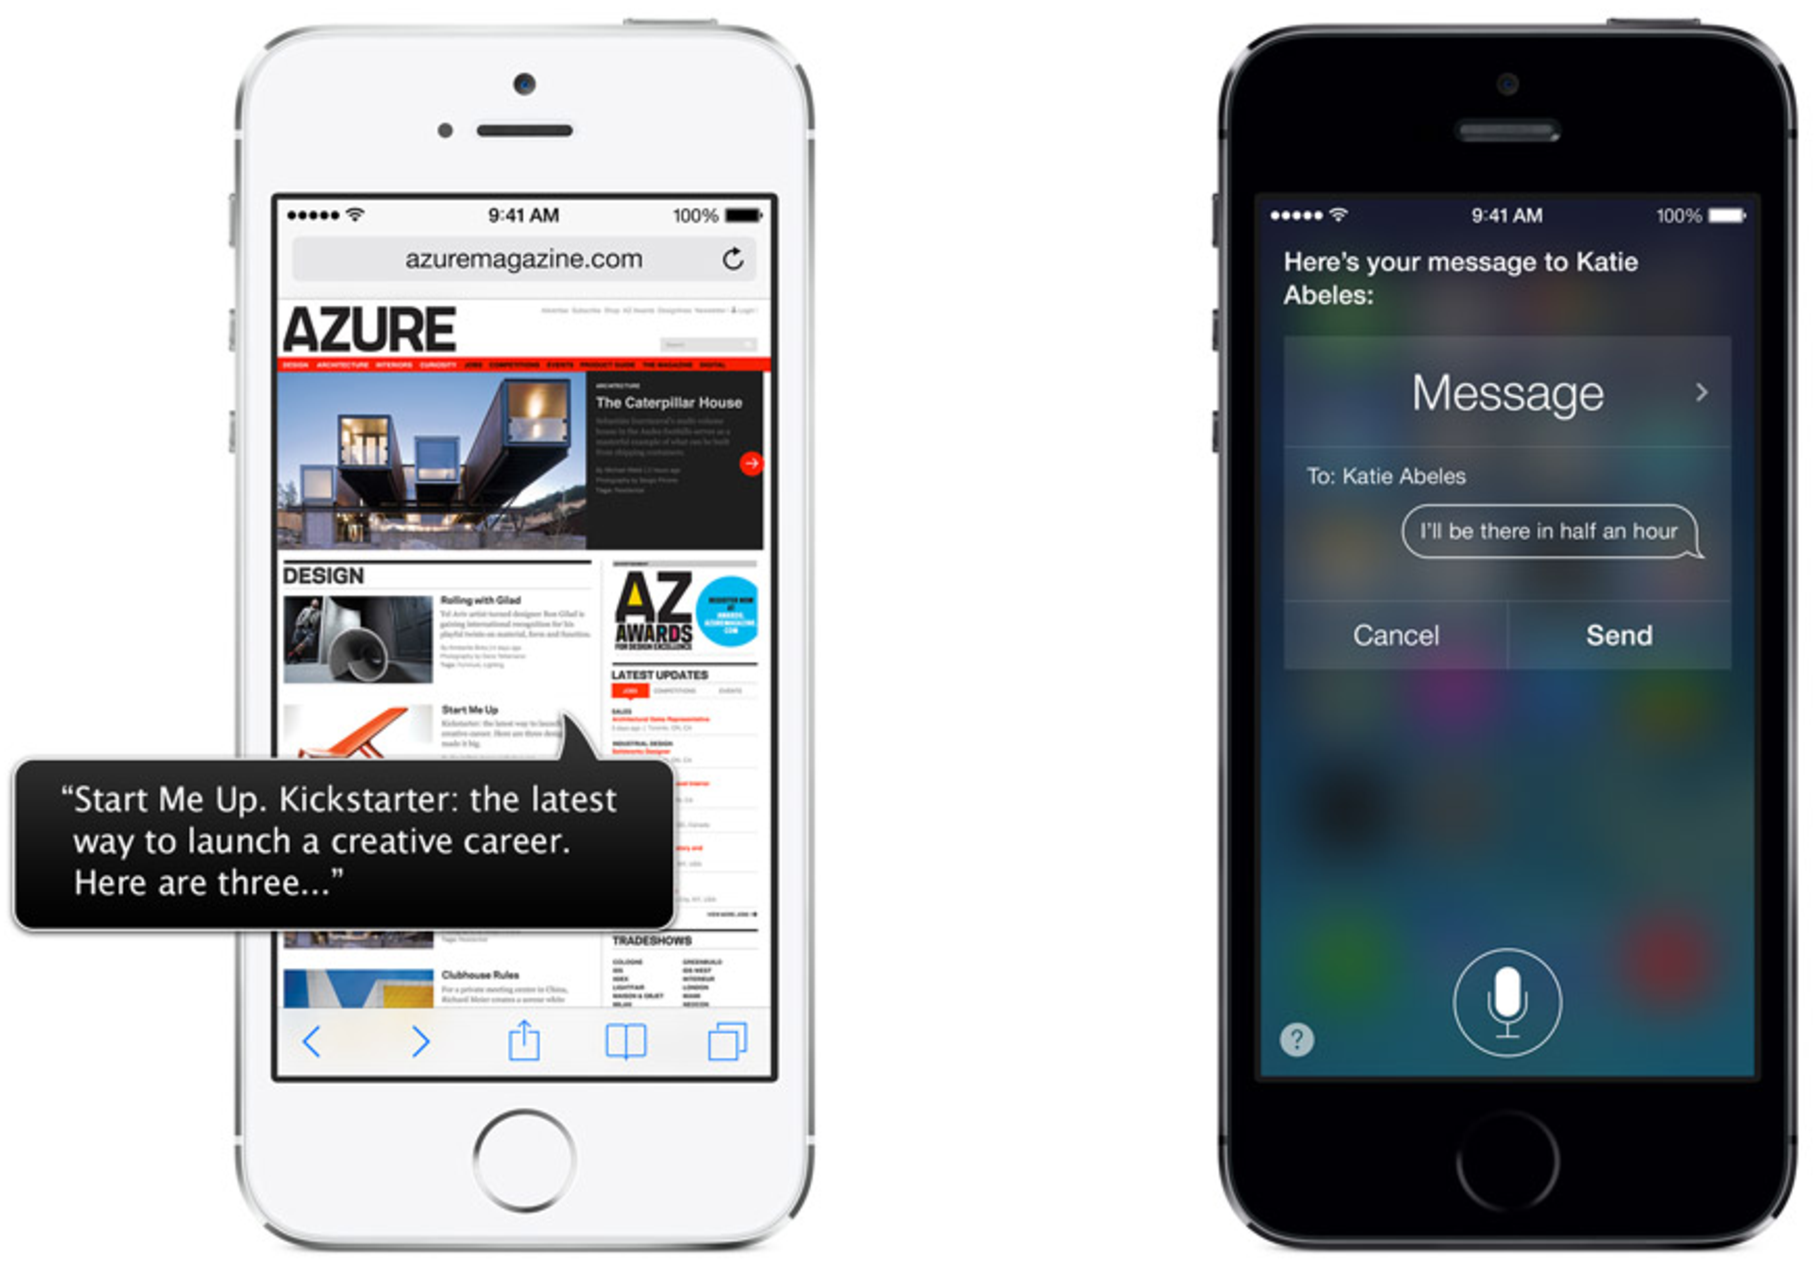
\includegraphics[width=0.7\textwidth]{accessibility_ios.pdf}
\caption{Several iOS accessibility tools~\citep{ios_accessibility}. On the left, 
VoiceOver~\citep{ios_voiceover}. On the right, Siri~\citep{ios_siri}.}
\label{fig:accessibility_ios}
\end{figure}

These accessibility functionalities make the user interfaces \textit{adaptable}
by the users. On the contrary, \textit{adaptive} user interfaces would modify 
the aspect of the shown elements without the user intervention. This means that 
adaptable user interfaces needs the user to change the corresponding adaptable 
characteristic (e.g., the font size) while an adaptive user interface would 
adapt without it.

Thus, once \textit{adaptable} and \textit{adaptive} concepts have been defined,
\textit{adaptivity} and \textit{adaptability} are introduced. \textit{adaptivity}
is related to the fact that a system or a service is able to learn somehow to 
change itself to increase the user satisfaction in the interaction process. 
On the other hand, \textit{adaptability} deals with the property of the system
or service to be customized by the user~\citep{jameson_modelling_2001}.

Now that we have defined what adaptivity means, several significant adaptive 
systems are presented in the following lines.

User interface adaptation has evolved through \ac{hci} history. First, and dealing with
the concept of adaptability (and not adaptivity), user interfaces start to be malleable. 
Colour palettes and screen resolution tools were given to the user. Nowadays, regarding
our portable devices, even automatic brightness control systems are available (dealing
with adaptivity). Since many years, developers have attempted to offer customization
tools to the end user. These tools have grown in complexity, covering a wider range of
functionalities and also users. What is more, a few years ago the context was taken
into account as the set of characteristics that define a situation.

Systems personalization and environment components adaptation has been demonstrated
to benefit both users and service providers~\citep{kobsa_generic_2001}. However, for
achieving a satisfactory adaptation it is necessary to have several inputs, for example,
a user characteristics model. Hence, the service provider will be able to apply the
corresponding adaptations for the corresponding user. Besides, we believe that current
context conditions~\citep{jameson_modelling_2001} and user's device capabilities are also
crucial within this domain. 
% In Section~\ref{sec:interaction_entities} we dig in
% this idea.

\citet{nilsson_model_based_2006} considered that designing user interfaces for
mobile devices tends to be problematic for several reasons (e.g., screen size is
small and interaction mechanisms are very different from a desktop system). Besides,
these devices are usually used in dynamic environments (i.e., variations in the
context). 

In the literature several context based user interface adaptation solutions can 
be found. Before reviewing them, it is necessary to first formally define context.
According to \citet{weerawarana_bean_2001} and \citet{dey_understanding_2001} 
context is defined as any situation that can be used to characterize the situation 
of an entity, taking an entity as a person, a place, or an object that is considered
relevant to the interaction between the user and the application (see
Section~\ref{sec:context}). The definition of \textit{use context} inherits from
the context definition itself as the set of variables values which models the
used device, so as the physical and social environment where the interaction is
being performed.

\citet{calvary_plasticity_2002} stated in 2002 that a user interface is \textit{plastic}
if it is capable to adapt itself taking into account context changes keeping
the usability. They presented a process and a dynamic software mechanism which
supports context variability. This work was supported by the idea that context
changes may provoke the triggering of several reactions under a \textit{prologue-action-epilogue}
paradigm. 
% In addition, to enhance the performance they introduced a
% \textit{historical of contexts}. By selecting pre-known configurations the
% adaptation process resulted faster. This historical database stores several
% context situations and the corresponding computed reactions. Besides, the
% \textit{''Plasticity Threshold"} and \textit{``Context Coverage"} novel concepts
% help to set the boundaries of a still valid user interface~\citep{calvary_supporting_2001}.

Using another paradigm,~\citet{lehtonen_dynamic_2002} detailed a tool to perform
dynamic adaptation on documents based on several user parameters (language,
document type, and so on). The presented approach is based on several \textit{configuration
files} (Product Configuration Files) which describe the current user interface and
store the user preferences. The user interfaces are designed with Bean Markup
Language~\citep{weerawarana_bean_2001} (a language focused on user interfaces)
and Java Beans.

Three \textit{middleware} based solutions are highlighted in the following lines.
\citet{repo_facilitating_2004} introduced in 2004 a model that allows the use 
of Web-based user interfaces (as well as the creation of new ones) that covers 
the environment adaptability requirements and context in the best possible way. 
The main problem is given by the range of devices that users typically employ, 
which have different capabilities and run different platforms. This situation 
causes the need of more flexible applications and devices. Repo identified a lack 
of attention in the initial adaptation process (e.g., when the capabilities of the
mobile device are identified). This approach was based on a \textit{middleware}
architecture, and it was capable of detecting new devices in the current environment
(context changes). It allowed services to query for devices' capabilities through 
a middleware architecture. Once a service identified a certain device, it sent 
the corresponding user interface. 

\citet{nilsson_model_based_2006} introduced a \textit{middleware} solution
which was able to build auto-adaptable systems. In this case, the middleware 
leads the adaptation process dynamically, providing several mechanisms to: 
detect changes in the application context, reason about these changes, and adapt 
to them by a dynamic reconfiguration of the current application. 

Based on the same architecture introduced by~\citet{nilsson_model_based_2006},
\citet{hallsteinsen_self_adaptation_2004} presented a system which was able to 
react to context changes recommending alternative configurations in each case.
The benefit for the user comes from the reasonable adaptation decisions took 
by the middleware, being the developer responsible for describing configuration 
options for important variation points.

\citet{stuerzlinger_user_2006} focused their work on desktop applications
adaptations and on the adaptation, reconfiguration and combination of user
interfaces using a \textit{User Interface Facades} system. Based on the definitions
laid down by~\citet{marmolin_medium_1995}, where differences between superficial
personalization (which allows users to select different options between some
predefined) and deep customization (which allows customizing deeper aspects of
the system) were introduced, authors stated the following criteria for adaptive
interfaces:

\begin{itemize}
  \item Fast, simple, or just-in-time customization: users are able to customize
  their interfaces without advanced planning, whenever they need it, and they will
  be able to do it in a simple way.
  \item Not only big personalization, also local ones (at minor scale).
  \item Deep personalization: users can define new customization rules.
  \item Cross-application personalization: interfaces customization must enable 
  different applications to be combined.
\end{itemize}

A \textit{framework} based approach is presented by~\citet{almeida_imhotep_2011}
in 2011. Imhotep is a framework for user interface adaptation based on inserting
preprocessor primitives within the source code. Thus, at compilation time
different versions of the final application are generated due to the corresponding
user and device parameters. A \ac{wurfl}~\citep{wurfl} database was used for modelling
devices and their capabilities. \ac{wurfl} is a \ac{ddr}, a catalogue of mobile 
device information and a framework for adaptation of mobile user interfaces.
By using it, authors ensure to have the latest devices with their capabilities.
As configuration files, the platform checks both user and device capabilities and
uses them to compile the corresponding solution. This approach has the limitation
of being static. This means that each change in the user capabilities needs a new
compilation of the whole application.

A work in progress by~\citet{evers_achieving_2012} et al. tackles the problem of
the need of user interaction in the adaptation process. Their work, centred in
users, discusses about adaptation versus usability defining different types of
adaptation (i.e., forward and backward) and different user ways of interaction
(i.e., implicit versus explicit). This perspective helps developers to take into
account not only technical characteristics (users models, devices capabilities,
context parameters, adaptation engines and so on) but also some psychology to be 
aware of user mood or stress. In stressful situations users may not be comfortable 
with an adaptation engine which asks questions about the process.

Several ideas of the reviewed works are taken into account for the proposed user 
model in combination with the~\citet{casas_user_2008} research. For instance,
the visual handicap metrics in the sensory layer gives an idea of modelling
not the user disability but the minimum needed configuration for a view component
in the screen. This issue is deeply discussed in Section~\ref{sec:user}.

\subsection{Physical Adaptive systems}
\label{sec:pyshical_adaptive_sistems}

Although it is out of the scope of this dissertation, there is a research
pathway dealing with physical adaptive systems. In Tactus~\citep{tactus}, a
company which aims to redefine devices and user experiences by combining the 
modern and traditional interfaces and on-demand buttons on touch
screens for a tactile experience~\citep{tactus_linkedin}, a novel adaptive
technology has been developed. This technology allow screens to dynamically build
physical buttons into a flat touch screen, depending on the current task. For example,
if the user needs to send an email, the keyboard emerges from the screen
as a physical interface. This interface is supported by the combination of
small fluid channels which are routed throughout the Tactile Layer. This layer
enables fluid to expand the top polymer layer to create the physical buttons (see
Figure~\ref{fig:tactus}).

\begin{figure}[H]
\centering
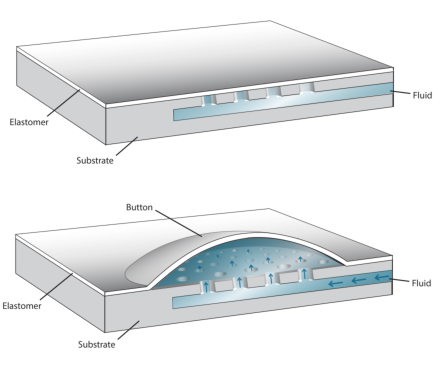
\includegraphics[width=0.55\textwidth]{tactus.pdf}
\caption{Buttons during the flat state (up) and during the raised state (down)~\citep{tactus}.}
\label{fig:tactus}
\end{figure}

Nowadays, this technology might be surprising for the reader. Nevertheless, there
are examples of physical user interfaces adaptation all around us. One of the most
common and spread example is shown in cars. The cars companies deal with adaptivity
for the current driver not just inside the car, but also outside. Some models
adapt the driving wheel in depth and height depending on the driver who unlocks
the door. Displays and controller brightness, even radio volume can be also
adapted considering context light or noise. Even the car lights system adapts
to the road conditions.

Again, these are just a few examples of what adaptation technologies might
be pointing to for the near future.

% ----------------------------------------------------------------------



% this file is called up by thesis.tex
% content in this file will be fed into the main document

%: ----------------------- introduction file header -----------------------
\begin{savequote}[50mm]
Personally, I think it does help, that it makes a beneficial difference, but the scientific literature on the subject is very messy.
\qauthor{Jeanne Petrek}
%“And upon the top of the pillars was lily work: so was the work of the pillars finished.”
%
% Bible quotes
\end{savequote}


\section{User Modelling}
\label{sec:user}

% the code below specifies where the figures are stored
\ifpdf
    \graphicspath{{2_state_of_the_art/figures/PNG/}{2_state_of_the_art/figures/PDF/}{2_state_of_the_art/figures/}}
\else
    \graphicspath{{2_state_of_the_art/figures/EPS/}{2_state_of_the_art/figures/}}
\fi


%------------------------------------------------------------------------- 

\subsection{A Chronological Review of the Evolution of User Models}
\label{sec:chronological_review}

Figure~\ref{fig:user_models} illustrates the chronological evolution and different 
solutions for the last 15 years. During these years different user characteristics 
have been taken into account considering the final purpose of the designed system. 

\vspace{1cm}
\setlength\taskwidth{1.7cm}

\begin{timeline}
  \label{chr:users}
  \Task[1991]{\citet{orwant_doppelgangeruser_1991}}
  \Task[1994]{\citet{brajnik1994shell}, \citet{paiva1994tagus}, \citet{kay1994toolkit}}
  \Task[1999]{\citet{pohl_logic_based_1999}}
  \Task[2001]{\citet{fischer_user_2001}, \citet{kobsa_generic_2001}.}
  \Task[2002]{\citet{gregor_designing_2002}}
  \Task[2003]{\citet{gauch_ontology_based_2003}, \citet{razmerita_ontology_based_2003}}
  \Task[2005]{\citet{hatala_ontology_based_2005}, \citet{pereira_triple_2005}, \citet{heckmann_gumogeneral_2005}}
  \Task[2007]{\citet{persad_characterising_2007}, \citet{golemati_creating_2007}}
  \Task[2008]{\citet{casas_user_2008}}
  \Task[2012]{\citet{evers_achieving_2012}, \citet{skillen2012ontological}}
\end{timeline}
\captionof{figure}{The chronological view of the evolution of remarkable user 
models considered in this dissertation.\label{fig:user_models}}


First user modelling systems started in the late eighties. 
\citet{allen_plan_based_1979},~\citet{cohen_elements_1979}, 
~\citet{perrault_speech_1978}, and \citet{rich_building_1979}\citep{rich_user_1979} 
are examples of researchers whose works inspired next user modelling approaches. 
From there, several authors started collecting different types of information 
about the users and exhibiting, for example, different kinds of adaptations to 
them~\citep{kobsa_generic_2001}.

Before overview the evolution of the user models, a definition of user modelling 
is needed. There are at least two different perspectives which might answer this 
question. One of these is related to \ac{ai}, and it considers user modelling 
as the process through which systems gather information and knowledge about 
users and their individual characteristics. Therefore, a user model is considered 
a source of information about the user of the system which contains several
assumptions about several relevant behaviour or adaptation data. However, in
this thesis the \ac{hci} research perspective is taken, which is defined by
\citet{pohl_logic_based_1999} as follows:

\begin{description}
  \item[\Defi{User Model, by \citet{pohl_logic_based_1999}}] \hfill \\
  \begin{mdframed}[hidealllines=true,backgroundcolor=gray!20]
  \textit{``It refers to an a-priori model of the users of a computer system that the system
  designer has in mind, or to the assumed models that users will probably develop
  of the system and the tasks they can perform using the system''}.
  \end{mdframed}
\end{description}

Nevertheless, this definition and the \ac{ai} perspective coincide in the idea that 
every system must use information about the user to be able to see and react to 
their different problems and needs and improve the system purpose. This section 
analyses the most significant user models in the past 15 years.

\subsection{User models}
\label{sec:user_models}

%sota user models
\subsubsection{1991: Jon Orwan and the Doppelgänger system}
\label{sec:orwant_doppelganger}

Doppelgänger is a user modelling system that performs inferences upon user data
and makes this information available to applications. The system allows users to
modify their models, it makes implicit generalizations about the data (which is
gathered through different channels) and provides an extensible architecture~\citep{orwant_doppelgangeruser_1991}. 

% ``Figure 1 The DOPPELGÄNGER user modelling system gathers data about users from sensors, makes inferences on
% those data, and makes the results available to applications'' cogido de http://www.cs.ucf.edu/~dcm/Teaching/COT4810-Spring2011/Presentations/FrankHines-CheapUserModelingForAdaptiveSystems.pdf

User data is gathered through a continuously operative sensor network which
senses users' everyday activities (see Listing~\ref{lst:orwant_sensor_1}). Hence,
both long-term and short-term information about the user are stored. Sensors are
integrated in users' activities. However, Doppelgänger acknowledges the imperfection
of real world data. Data streams are usually incomplete or erroneous. The main
objective of the Doppelgänger system is to recover from these imperfections through
several learning techniques:

\begin{itemize}
  \item The Beta distribution~\citep{drake_fundamentals_1967}, which is used to
  determine the preference strength, probability of accuracy and the confidence
  of an estimation.
  \item Linear prediction, to predict a possible next event.
  \item Markov models, which represents user's behaviour through several states and
  all possible transitions between them with the corresponding probability.
\end{itemize}


The system maintains an accuracy estimation for each sensor, which helps the
system to decide a confidence metric for the gathered data.

\begin{minted}[linenos=true, fontsize=\footnotesize, frame=lines]{json}
(object orwant location (place 344) (time 779562701) 
(id active-badge))
\end{minted}
\captionof{listing}{Message from a sensor to the server~\citep{orwant_heterogeneous_1994}.\label{lst:orwant_sensor_1}}


The user models are represented in SPONGE, a LISP based data structure manipulated with
C and Pearl programs \citep{orwant_heterogeneous_1994} (see Listing~\ref{lst:orwant_sensor_2}). 
Models are stored as Unix directories consisting of domain submodels and conditional 
submodels. The first one contains information about the user behaviour (i.e., 
location, preferences, and so forth); the second group contains triggering information 
for deciding actions when certain situations are met. Besides, each user model 
is conceptually represented as a point in a high dimensional space in which the 
dimensions are determined by the number of sensors in the network.


% \InsertFig{orwant}{fig:orwant}{Orwant user model \citep{orwant_heterogeneous_1994}}{}{0.70}{}
% 
% \InsertFig{orwant}{fig:orwant_sensors_apps}{The DOPPELGÄNGER user modelling system gathers data about users from sensors, makes inferences on
% those data, and makes the results available to applications. \citep{orwant_for_1996}}{}{0.70}{}

\begin{minted}[linenos=true, fontsize=\footnotesize, frame=lines]{json}
(object orwant primary
  (object biographical_data
    (string_binding "true name" "Jon Orwant")
    (string_binding "e-mail address" orwant@media.mit.edu)
  ...)
  (object control
    (int_binding "doppelganger ID" 4))
...)
\end{minted}
\captionof{listing}{Orwant user model~\citep{orwant_heterogeneous_1994}.\label{lst:orwant_sensor_2}}

% \begin{figure}
% \centering
% \includegraphics[width=0.7\textwidth]{orwant_sensors_apps.pdf}
% \caption{The DOPPELGÄNGER user modelling system gathers data about users from sensors, makes inferences on
% those data, and makes the results available to applications~\citep{orwant_for_1996}.}
% \label{fig:orwant_sensors_apps}
% \end{figure}
% ----------------------------------------------------------------------


\subsubsection{2001: Gerhard Fischer}
\label{sec:fischer_user_2001}

In 2001~\citet{fischer_user_2001} reviews the user models of the past 10 years. 
He describes how using computers in \ac{hci} environments has been always
modelled as a user-computer couple. These elements are modelled as an explicit 
connection which represents the communication between them. New and modern 
interfaces such as windows, menus, pointers, colours, sound and touch screens 
have enlarged this communication line thanks to their capabilities.

Furthermore, in addition to the possibilities of new design approaches,
knowledge-based architectures in \ac{hci} explore the possibility of implicit
communication channel. The required knowledge considers the problem domain,
communication processes and the communication agent. Users are part of the
communication agent group. Fischer defends the idea that there are many types of
users. Besides, their needs change with the experience and through time.
Hence, a simple user classifications (e.g., \textit{novel}, \textit{intermediate}
and \textit{expert}) is not enough to characterize users in complex environments. 
Nevertheless, despite Fischer remarks the significance of each agent, he does 
not establish which agent capabilities are important to face the problem of 
modelling a user.

% \InsertFig{fischer}{fig:fischer}{The human-computer interaction channel 
% \citep{fischer_user_2001}}{}{0.70}{}

\begin{figure}
\centering
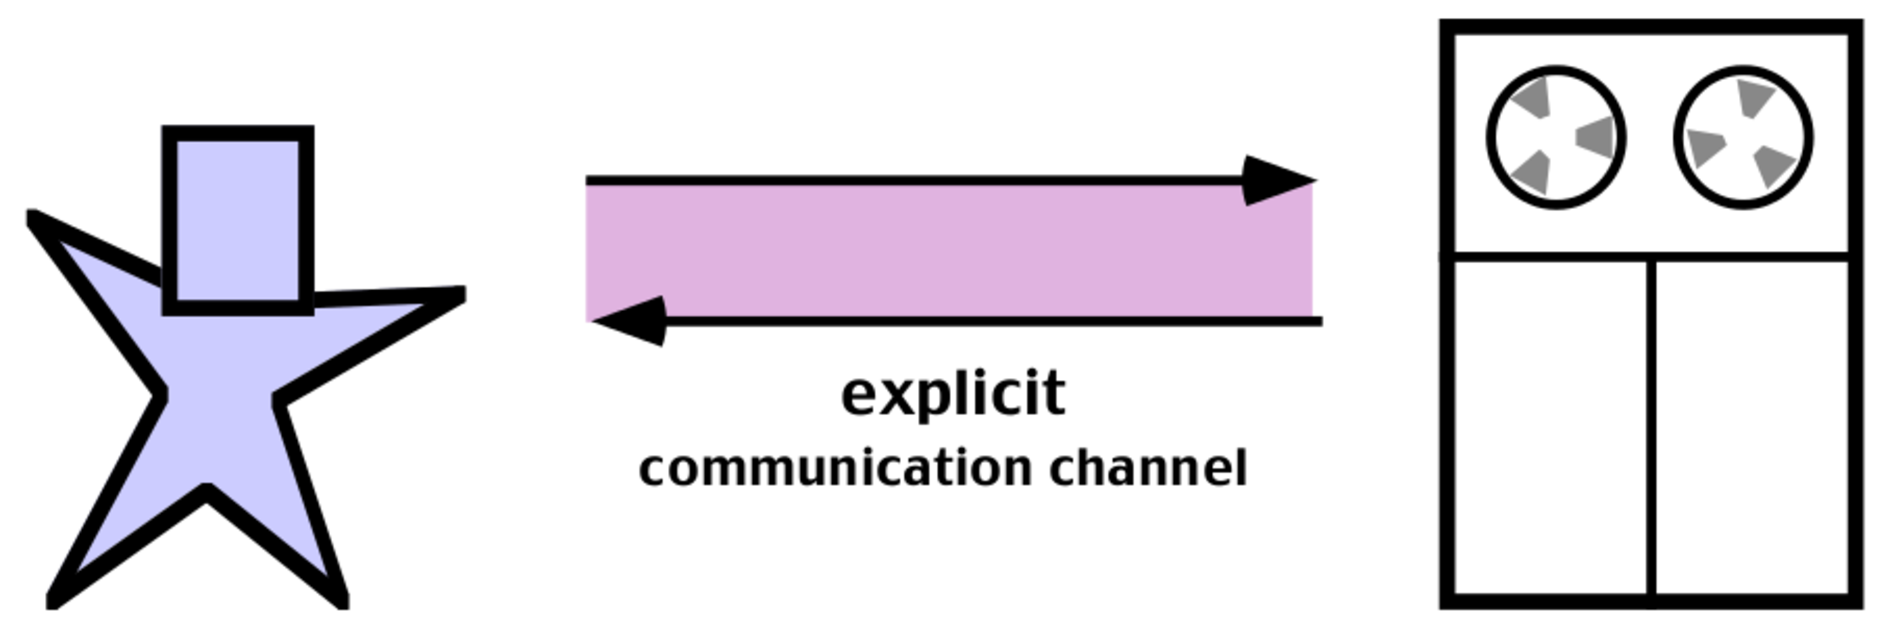
\includegraphics[width=0.50\textwidth]{fischer.pdf}
\caption{The \ac{hci} channel~\citep{fischer_user_2001}.}
\label{fig:fischer}
\end{figure}
\subsubsection{2002: Gregor et al.}
\label{sec:gregor}

%------------------------------------------------------------------------- 
In 2002,~\citet{gregor_designing_2002} focus their approach on a certain groups 
of users: the elderly. A three group classification is presented. In the first 
group there are the fit older people, who do not suffer from any disability. The 
second group is formed by older fragile people who have one or more 
disabilities. Finally, the last group encompasses the older and people with 
disabilities whose capabilities to function depend on other people. In this 
case, the authors identify several user capabilities:

\begin{itemize}
 \item Physical, sensory and cognitive capabilities.
 \item The ability to learn new techniques (cognitive).
 \item Memory problems (cognitive).
 \item The environment can affect several elderly capabilities.
 \item Elderly experience (as a positive fact).
\end{itemize}

On the other hand,~\citet{gregor_designing_2002} consider that, as people grow 
older, their capabilities change. This process encompasses a reduction of 
cognitive, physical and sensory functions depending on the individual. This 
diversity is a significant issue for modelling users and designing computing 
systems.

Figure~\ref{fig:gregor} shows an adaptable user interface which takes into 
account these capabilities. 

% \InsertFig{gregor}{fig:gregor}{Adaptable browsing 
% interface~\citep{gregor_designing_2002}}{}{0.70}{}

\begin{figure}
\centering

\includegraphics[width=0.70\textwidth]{gregor.png}
\caption{Adaptable browsing 
interface~\citep{gregor_designing_2002}.}
\label{fig:gregor}
\end{figure}

\subsubsection{2003: Gauch et al.}
\label{sec:gauch}

Towards the goal of personalized navigation of online information~\citet{gauch_ontology_based_2003}
provide a user ontology for dynamically modelling the user browsing. The ontology
is formed by several concepts which are weighted indicating the user's perceived
interest in the corresponding concept. These concepts are related with surfing
experience (i.e., the content, length and time spent) on each Web page and
classified into the reference ontology. Hence, the user profile is created 
automatically. This means that the user profile information is collected 
implicitly without user feedback, as the ontology's concepts are automatically 
weighted considering the amount of related information from the user browsing.


% ----------------------------------------------------------------------

\subsubsection{2003: Razmerita et al.: The OntobUM Ontology}
\label{sec:razmerita2003ontology}

Focused in the context of \ac{kms}~\citet{razmerita_ontology_based_2003} present
OntobUM, a generic ontology-based architecture for user modelling. The model is 
generated through two different ways:

\begin{itemize}
  \item Explicitly, using a user profile editor. Thus, the user has to 
  provide some information.
  \item Implicitly, information maintained by several intelligent services 
  which maintain and update the information about the user considering the 
  user's behaviour with the services and provide adapted services based on 
  user's preferences.
\end{itemize}

The architecture of the presented ontology is composed of the following ontologies:

\begin{itemize}
  \item The User Ontology, which structures the different characteristics and 
  preferences of the user.
  \item The Domain Ontology, which defines several concepts about the domain.
  \item The Log Ontology, which manages the semantics of the interaction 
  between the user and the whole system.
\end{itemize}

Authors identify several users' characteristics that are relevant for a \ac{kms} 
under the Behaviour concept. Nevertheless, most of the user ontology is 
generic and it is available to be used in other application domains. 

%Dynamic user modeling? Atención al proceso de captura de datos implícita.

\subsubsection{2005: Hatala and Wakary and the Ec(h)o system}
\label{sec:hatala}

Ec(h)o is an ontology-based augmented audio reality system for museums which 
aims to maintain rich and adaptive output information. The main purpose of this 
work is to address the problem of supporting experience design and functionality 
related to museum visits through user models combined with augmented reality 
and tangible user interface system.~\citet{hatala_ontology_based_2005} find
several challenges for capturing rich context information. For the presented 
museum scenario, social, cultural, historical and psychological factors are 
significant for the user experience. In this field, the argumentation made by
is remarked as relevant. \citeauthor{dourish_what_2004} states that activities 
and context are directly and dynamically linked \citet{dourish_what_2004}\citep{dourish_where_2004}.
This concept is called \textit{embodied interaction}.

The core of the ec(h)o's reasoning module is a dynamically updated user model
\citep{wahlster1989user}. The ruled-based model changes as the user moves 
through the museum and selects several audio objects. This models enables 
developers to consider which inputs influence user interests. In the ec(h)o 
system there are two ways of updating the model: the user movement and a 
selection of an audio object. These actions have different effects on the model 
of the user interests (i.e., influence of initial interest selection, of object 
selection on user interest and of location change). 

As it occurs with recommender systems, user's interest are vital for the concept
ontology. These concepts are weighted in the ontology as concepts which represent
the user's likes within the environment. Besides, an interaction history is 
maintained recording the way the user interacts with the museum. In addition to 
these characteristics the user type is also considered. Hence, the system is 
allowed to characterize the user experience with the environment. It classifies 
users into three different categories:

\begin{itemize}
  \item The \textit{avaricious} visitor, who wants to see as much as possible
  in a sequentially way.
  \item The \textit{selective} visitor, who is more selective with the concepts 
  he/she is interested in.
  \item The \textit{busy} visitor, who prefers to not spend much time and get a 
  general vision of the exhibition.
\end{itemize}

\subsubsection{2005: Fernando Pereira}
\label{sec:pereira}

Within a video adaptation and quality of experience evaluation scenario,
~\citet{pereira_triple_2005} studies a user characterization through three
different dimensions: sensory, perceptual and emotional. First of all,
\citeauthor{pereira_triple_2005} establishes the difference between sensations 
and perceptions as follows:

\begin{itemize}
  \item \textit{Sensations} are monomodal, more low-level, physical and less 
  related to the real world composition than perceptions. They regard the simple 
  conscious experience for the corresponding physical stimulus (e.g., light 
  variation and eyes reaction to this change). They are related to the first 
  contact between a human and the surrounding environment.
  
  \item \textit{Perceptions} are multimodal, and they are part of the cognition 
  process (knowing and learning) and regard the conscious experience and 
  identification of objects.
\end{itemize}

On the other hand, emotions are considered as central in a communication and 
entertainment process. Therefore, \citeauthor{pereira_triple_2005} proposes a 
triple layered \ac{spe} user model for the evaluation of the quality of 
experience in the consumption of multimedia content.





\subsubsection{2007: Heckmann et al.}
\label{sec:heckmann}

A different approach is implemented by~\citet{heckmann_gumogeneral_2005}.
Divided into four main groups (emotional state, personality, characteristics and
physiological state), the authors present the \acf{gumo}, an ontology model to 
characterize users capabilities within adaptive environments. A significant 
user aspect that is taken into account in this work is the stress. In the 
adaptive interfaces domain it is needed to pay special attention to the 
consequences of each adaptation. But the stress is not only determined  by this 
process. It is also derived from several user experiences, as the current 
context state (e.g. traffic, noise, surrounding people, and so 
forth~\citep{babisch_noise_stress_2002}). Figure~\ref{fig:heckmann_model} illustrates
the model presented by~\citeauthor{heckmann_gumogeneral_2005}.

% \InsertFig{heckmann_model}{fig:heckmann_model}{Several user model property
% dimensions~\citep{heckmann_gumogeneral_2005}}{}{0.70}{}

\begin{figure}
\centering
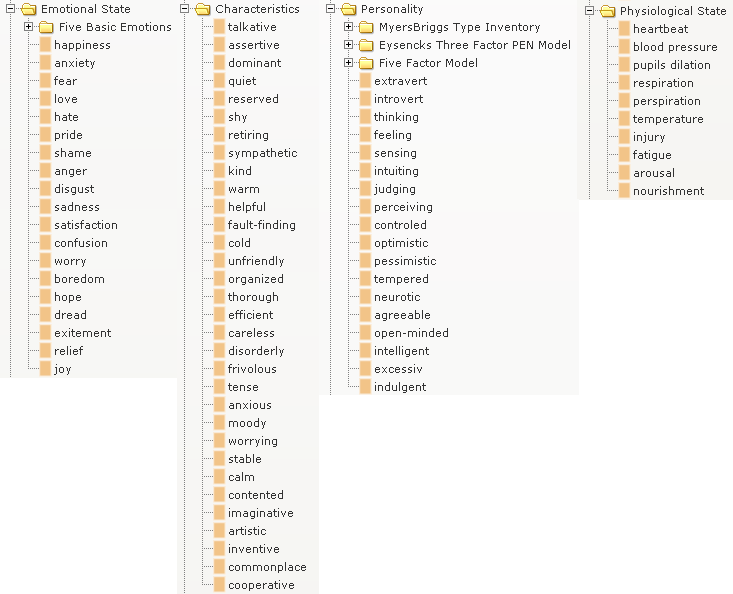
\includegraphics[width=0.70\textwidth]{heckmann_model.png}
\caption{Several user model property
dimensions~\citep{heckmann_gumogeneral_2005}.}
\label{fig:heckmann_model}
\end{figure}

% ----------------------------------------------------------------------

\subsubsection{2007: Persad et al.}
\label{sec:persad}

\citet{persad_cognitive_2007}\citep{persad_characterising_2007} relate user
capabilities and product demands as a tool to evaluate the product design (see Section~\ref{sec:motivation}).
\citeauthor{persad_characterising_2007} remark four main components to consider 
when dealing with interaction between people and technology: the user, the 
product, the environment or context, and the set of activities or tasks 
that define the interaction. The authors try to assess an adaptation degree 
between users and the designed products using different compatibility measures. 
These measures can be assessed on different levels of human capabilities, 
including sensory, cognitive and motor. The concepts of user capability and 
product demand provide a useful framework for analysing the user-device 
compatibility. The product demand levels are considered multidimensional and 
they are set by the interface attributes of the product itself. For example, 
a product's text display will be designed with a certain text size, font, and 
colour contrast. The combination of these attributes define the visual demand 
level within the user visual capabilities. Similarly, other combinations of 
product attributes command several cognitive and motor demands. 

\citeauthor{persad_cognitive_2007} also reviewed functional classifications 
and experimental studies to identify the most relevant low-level skills for 
designing products within the cognitive, motor and sensory domain. This is 
highly related to the \ac{icf} functions described in Section~\ref{sec:background_icf}.

\paragraph*{Sensory capabilities}
\subparagraph*{Visual capabilities:} Several sensory capabilities are known to 
deteriorate with ageing~\citep{persad_exploring_2006}. Thus, 
\citeauthor{persad_exploring_2006} state that the following functions seem to 
account for most of visual disability:

\begin{itemize}
  \item Visual acuity.
  \item Contrast sensitivity.
  \item Colour perception.
  \item Useful field of view.
  \item Stereopsis.
\end{itemize}


\subparagraph*{Hearing capabilities:} Loss of hearing capabilities may directly 
affect the speech interaction with the device. The main low-level hearing 
functions to guarantee the interaction are the following:

\begin{itemize}
  \item Pure tone detection thresholds.
  \item Speech detection and recognition discrimination thresholds.
  \item Sound localization.
\end{itemize}

% \subparagraph*{Environmental effects}
% The level of illumination, noise, weather, etc. are several environment features 
% which might affect user capabilities.

\paragraph*{Cognitive capabilities}
The product's user interface must be usable and accessible enough to guarantee 
that users easily understand the interaction. The following capabilities are 
related to the human cognitive domain:

\begin{itemize}
 \item Working memory performance.
 \item Long term memory.
 \item Mental models, planning and problem solving.
 \item Language and communication capabilities.
\end{itemize}

\paragraph*{Motor capabilities}
\subparagraph*{Upper limb capabilities:}
There are many conditions that affect manipulating a product (e.g., arthritis, 
stroke, multiple sclerosis, head injury, cerebral palsy and missing or damaged 
limbs). These problems directly reduce grasp forces, range of motion and fatigue 
thresholds~\cite{persad_characterising_2007}.

The following areas are highlighted within motor capabilities:
\begin{itemize}
  \item Reach ranges for each arm.
  \item Grasping, dexterity and force exertion.
  \item Two handed actions and coordination.
\end{itemize}

\subparagraph*{Gross body movement capabilities:}
Usually products require certain user mobility degree. 

\bigskip

Besides, \citeauthor{persad_characterising_2007} provide six general categories 
for product features and their interface classification. For this classification 
their toaster case study is considered, \textit{``which is used to demonstrate 
the capability-demand interaction''} (see Table~\ref{tbl:persad_product_interface}).

\begin{table}
  \caption{Product interface classification by~\citet{persad_characterising_2007}.}
  \label{tbl:persad_product_interface}
\footnotesize
\centering
    \begin{tabular}{l l}
    \hline
    \textbf{Feature type} 	& \textbf{Examples} \\
    \hline
    Product chassis 		& Handles, gripping surface. 		\\
    Displays and indicators 	& Visual and auditory displays. 	\\
    Controls and control groups & Discrete controls (button, switch) 	\\
				& and continuous controls (slider,  	\\
				& knob, thumb, wheel, dial, joystick).	\\
				& Control groups \textit{Keypad}. 	\\
    Material/media input 	& Slots (toaster slots), powered and 	\\
    and output			& un-powered bays and trays, doors, 	\\
				& lids and covers.			\\
    Connectors for energy and data & Power and data connectors 		\\
    Software interfaces 	& Navigation menus and \ac{gui} objects. \\
    \hline
  \end{tabular}
\end{table}



\subsubsection{2007: Golemati et al.}
\label{sec:golemati2007creating}

\citet{golemati_creating_2007} present an ontology which considering past 
literature solutions aims to reduce the intrinsic problems of user modelling: 
ad-hoc modelling processes, the required amount of work to model users and the 
possibility of errors by omitting several user's characteristics. To this end,
the authors present an extensible, comprehensive and general ontology whose design
is addressed through a top-down approach by firstly collecting static information
about the user. Next, the ontology designers analyse the semantics of the profile
models and suggest concepts that would adequately model them. It is remarkable
that this work is focused on static user characteristics, although they consider 
the possibility of incorporating dynamic and temporal characteristics.

%Muy importante que modela características. Esto va directo a la parte de discussion de los modelos de usuario





\subsubsection{2008: Casas et al.}
\label{sec:casas}

Another approach is the one presented by~\citet{casas_user_2008}. In this case 
the authors work under the \textit{Persona} concept which is introduced to 
distinguish different user groups within an adaptive user interfaces domain. 
Originally this concept was introduced by \citeauthor{cooper_inmates_2004} in 
1999 by the following definition:

\newpage

\begin{description}
  \item[\Defi{Personas, by \citet{cooper_inmates_2004}}] \hfill \\
  \begin{mdframed}[hidealllines=true,backgroundcolor=gray!20]
  \textit{``Personas are not real people, but they represent them through a design 
  process. They are hypothetical archetypes of real users''}. 
  \end{mdframed}
\end{description}

\citeauthor{casas_user_2008} distinguish between two categories of people:

\begin{itemize}
 \item \textit{Primary}: those who represent the main group and use primary 
 interfaces. 
 \item \textit{Secondary}: those who can use primary interfaces, but with 
 several extra needs.
\end{itemize}

By assigning random values to several characteristics (e.g., age, education,
profession, family conditions, disabilities and technological experience) 
authors are capable of covering a wide range of potential users. However, the 
most significant contribution is that, instead of being focused on users 
capabilities, they consider users needs. To that end they build a user 
profile supported by four main bases: 

\begin{itemize}
 \item The user level, which indicates the ability of the user to face the 
 system.
 \item Interface, for the interaction mechanism to be used by the user.
 \item Audio, to indicate the audio volume levels.
 \item Display, which includes usual display controls (contrast, colours, 
 brightness and so on).
\end{itemize}

This approach is focused on the solution, on the adaptation itself. It is a 
perspective which allows users to configure the interaction based on their 
capabilities. This helps applications designers because user capabilities are 
not directly taken into account in the model as medical or technical aspects. 
Hence, there is no need to be experts or have any physiological knowledge or 
experience about users disabilities. Another advantage is that each user can 
manage his/her own profile. Thus, they can configure their preferences and 
capabilities on their own. 

\subsubsection{2012: Evers et al.}
\label{sec:evers}

Several studies, as the research presented by~\citet{evers_achieving_2012},
recognize that it is complex to perform interfaces adaptations without bothering
the user. On the one hand, adapting an interface without the participation of the
user might lead to an unsatisfactory result. On the other hand, asking too much
for participation might bother the user. 
% From this work we assume that if the user
% has high stress levels the corresponding application should not ask for interaction.
% This way, the application should operate as ``automatic'' and 
% ``self-sufficient'' as possible. 
Following this stress perspective~\citet{liao_decision_2005} present an unified 
probabilistic decision model based on Influence Diagrams for modelling user stress 
levels. These levels were inferred by probabilistic inferences of several sources 
data (e.g., heart rate, mouth openness, head movements, or pupils monitoring).


\subsubsection{2012: Skillen et al.}
%\citep{skillen2012ontological}
\label{sec:skillen}

Within an application personalization within mobile 
environments~\citet{skillen2012ontological} present a User Profile Ontology 
which is able of modelling dynamic components. The ontology considers both 
static and dynamic aspects of the user mainly focused on his/her behaviour 
changes. The user capabilities are also taken into account for the user profile. 
Capabilities are defined as the extent to which the user has an ability (i.e., 
physical, emotional or cognitive) to carry out some activities. User's interests 
and several context parameters are also considered in the ontology to cover 
context-aware environments. Figure~\ref{fig:skillen_ontology} overviews the 
User Profile Ontology classes, object properties and data properties presented 
by~\citeauthor{skillen2012ontological}.

\begin{figure}
\centering
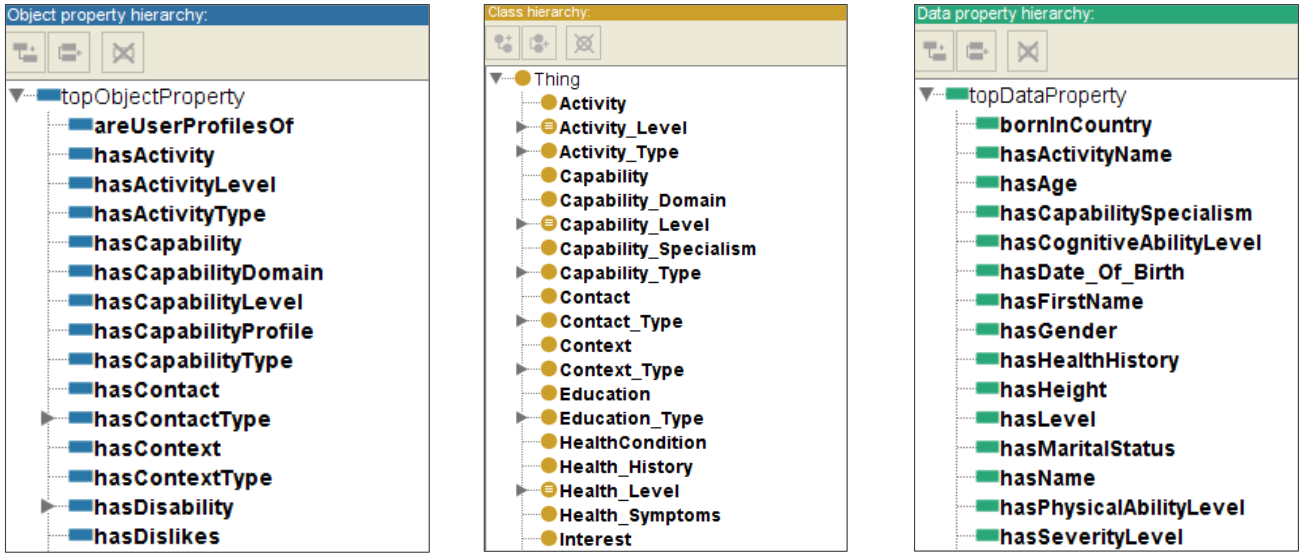
\includegraphics[width=0.70\textwidth]{skillen_ontology.png}
\caption{An overview of the User Profile Ontology classes, object properties and 
data properties~\citep{skillen2012ontological}.}
\label{fig:skillen_ontology}
\end{figure}

\subsubsection{Generic User Modelling Systems}
\label{sec:generic_users}

Apart from the analysed models there is another generic approach for modelling 
users known as Shell Systems. More focused in the field of \ac{ai}, these 
solutions consider the user model as a source of information which are built on 
assumptions about relevant user aspects or 
behaviour~\citep{pohl_logic_based_1999}.

\citet{heckmann_ubiquitous_2005} differentiates between the model, which is where 
the user data is collected, and the modelling system, which is the module that
manages the model. Besides, he remarks the following two definitions
from~\citet{wahlster_user_1989} previous work:

\begin{description}
  \item[\Defi{User Model (I), by~\citet{heckmann_ubiquitous_2005}}] \hfill \\
  \begin{mdframed}[hidealllines=true,backgroundcolor=gray!20]
  \textit{``A user model is a knowledge source in a system which contains explicit
  assumptions on all aspects of the user that may be relevant to the behaviour
  of the system. These assumptions must be separable by the system from the
  rest of the system's knowledge''}~\citep{wahlster_user_1989}.
  \end{mdframed}

  \item[\Defi{User Model (II), by~\citet{heckmann_ubiquitous_2005}}] \hfill \\
  \begin{mdframed}[hidealllines=true,backgroundcolor=gray!20]
  \textit{``A user modelling component is that part of a system whose function is to
  incrementally construct a user model; to store, update and delete entries;
  to maintain the consistency of the model; and to supply other components of
  the system with assumptions about the user''}~\citep{wahlster_user_1989}.
  \end{mdframed}
  
\end{description}


% % \begin{framed}
%   \begin{mydef}
%     {A user model is a knowledge source in a system which contains explicit
%     assumptions on all aspects of the user that may be relevant to the behaviour
%     of the system. These assumptions must be separable by the system from the
%     rest of the system's knowledge.~\citep{wahlster_user_1989}}
%   \end{mydef} 
% % \end{framed}
% 
% % \begin{framed}
%   \begin{mydef}
%     {A user modelling component is that part of a system whose function is to
%     incrementally construct a user model; to store, update and delete entries;
%     to maintain the consistency of the model; and to supply other components of
%     the system with assumptions about the user.~\citep{wahlster_user_1989}}
%   \end{mydef} 
% % \end{framed}

Assumptions are deeply studied and depicted in~\citep{pohl_logic_based_1999}. 
In this section, a quick overview of how these systems behave is performed to 
just take into account the difference between generic user modelling approach 
(user modelling shells) and the approach followed in this dissertation, which 
is related to Human-Computer Interaction.

In 1986 \ac{gums} is presented. This software allowed developers to make 
user-adaptive applications by defining several stereotypes, facts and rules to 
reason with~\citep{finin_gums_1986}. \acs{gums} supports the addition of new 
facts in runtime, manages facts inconsistencies and answers the application 
about assumptions about the user~\citep{kobsa_generic_2001}. The following 
systems are several examples of generic user systems developed in the following 
years (chronological ordered):

\begin{itemize}
  \item DOPPELGÄNGER, which uses several learning techniques for generalizing
  and extrapolating sensor data for the development of the user model
  \citep{orwant_doppelgangeruser_1991}.
  \item \ac{umt}, which supports the definition of hierarchically ordered 
  stereotypes about the user, rules for user model inferences and contradiction 
  detection~\citep{brajnik1994shell}.
  \item TAGUS, which uses first-order formulas to represent assumptions about
  the user~\citep{paiva1994tagus}.
  \item The um toolkit, which models not only assumptions but beliefs, preferences and other
  user characteristics in attribute-value pairs~\citep{kay1994toolkit}.
  \item BGP-MS, which permits user and groups of users assumptions~\citep{kobsa1994user}.
\end{itemize}

% MÁS SISTEMAS? SOLO LLEGAMOS A 1995\dots ESTOS SISTEMAS SON MUY ANTIGUOS, SI NO PONEMOS A
% PARTIR DEL 2000 MEJOR NI PONERLOS IGUAL\dots


% A significant aspect of these systems is that they are required to be usable in
% as many applications as possible. This is, domain independent. Therefore, they
% are expected to provide as many services as possible. On the contrary, in Human-Interaction
% user modelling approaches this is, in fact, an issue \citep{cita_falta_modelos_usuarios_comparar}.
% This problem is addressed in Chapter~\ref{cha:el_que_sea}.

% Domain independence
% 
% Known systems: 
% 
% GroupLens
% LikeMinds
% Personalization Server
% Frontmind
% Learn Sesame

% \InsertFig{heckmann_model}{fig:heckmann_model}{Several user model property dimensions \citep{heckmann_user_2007}}{}{0.70}{}

% ----------------------------------------------------------------------



\subsection{Users Models Comparison}
\label{sec:user_model_comparison}

In this section we describe our user modelling requirements nurtured by the 
earlier works described. As mentioned before, there are several perspectives 
regarding the user modelling requirements. In this dissertation the \ac{hci} 
perspective is taken. This means, as~\citet{pohl_logic_based_1999} states, 
that the user model refers to user characteristics using a certain system (see 
Section~\ref{sec:chronological_review}). In Chapter~\ref{cha:ontology_model}
the AdaptUI models for user, context and device are described. These models
have been designed considering each of these entities as a set of characteristics
that define them. Hence, the adaptation platform is able to evaluate the
combination of these characteristics and perform the corresponding adaptation.
Thus, the \ac{hci} interpretation of user modelling suits the goal pursued
by AdaptUI.

% Now that the \ac{hci} viewpoint has been remarked, we emphasize the amount of 
% different domains that are addressed in the literature considering user 
% modelling. 

In the following lines the amount of different domains addressing user modelling 
are highlighted. From product design to multimedia and user interfaces adaptation, 
every approach follows the same purpose: to consider several user characteristics 
to improve the system and user's satisfaction and product or service usability. 
However, although these solutions share the same objectives, the considered 
characteristics differ a lot. For ubiquitous and more context-aware domains, 
activities are taken into account. For example,
~\citet{razmerita_ontology_based_2003} discuss an ontology based architecture, 
which aims to be generic by collecting user data through two different ways 
(explicitly and implicitly).~\citet{golemati_creating_2007} also take an 
ontological point of view to avoid the problem of domain dependency (among 
others) by designing a more general, comprehensive and extensible ontology. 

\citet{gauch_ontology_based_2003} remark in the presented ontology the 
importance of time. Regarding the studied domain (web browsing) time is 
significant because it might help characterizing the user considering the spent 
time reading an article or visiting a website. Well known and popular 
recommendation systems, as YouTube, utilise this information combined with 
different explicit and implicit sources from the user interaction to make proper
recommendations~\citep{davidson_youtube_2010}.

User activities have also been considered as relevant for many authors in the 
literature. The first example is the Doppelgänger 
system~\citep{orwant_doppelgangeruser_1991} (1991), which uses activities for 
sharing relevant user information to different applications. In the same 
way,~\citet{persad_characterising_2007},~\citet{heckmann_gumogeneral_2005}
and~\citet{skillen2012ontological} modelled activities to take user's behaviour
and interaction into account for the proposed classifications and systems. For
~\citet{hatala_ontology_based_2005} activities are also vital within 
context-aware environments.

As occurs with context modelling (see Section~\ref{sec:context_model_comparison})
many different techniques are available for the model representation. This usually
depends either on the developer, because of his/her experience, or in the system's
technical characteristics. For example, if the system is able to performs inference
with the user data an ontology based representation could be more helpful than
an object based one.~\citet{strang_context_2004} demonstrated that ontological
modelling is more appropriate for ubiquitous computing environments.

It is also common to model physiological related characteristics of the user.
For example, the works by~\citet{gregor_designing_2002} 
and~\citet{persad_characterising_2007} consider physical, cognitive an sensory 
capabilities.~\citet{skillen2012ontological} also model several user abilities 
for performing different tasks and activities. The problem is that being aware 
of these capabilities is difficult and, in some cases, poorly practical. For 
example, measuring the sight capability of one individual requires physiological 
experience or advice. Besides, people with the same affection do not respond in 
the same way. A person who was born blind would interact differently with the 
environment than another who has been losing sight during his/her life. The 
precise same disability (e.g., tunnel vision) might affect different people 
in many different ways depending on their personal skills (e.g., adaptability,
orientation, and so forth). This might lead to an idea. What if, instead of 
modelling physiological skills (disabilities), we were able to model user's 
capabilities? The first approximation for this is found 
in~\citet{casas_user_2008} work. \citeauthor{casas_user_2008} present a user 
profile which abstracts from physiological aspects and lets users manage and 
configure their own profile. On the contrary, \citet{skillen2012ontological} 
model user capabilities as a set of abilities which allow users to perform some 
task or activities. Although this perspective covers many user capabilities, it
still needs a deeper understanding of physiological user capabilities.

On the other hand,~\citet{fischer_user_2001} comments that it not only is 
difficult to model users because of the wide range of different types of people 
that exist. He also considers that each individual changes with experience and 
through time. For example, old people's capabilities decrease with ageing. This
idea is shared with~\citet{gregor_designing_2002}, whose work is centred around
the elderly. \citet{heckmann_ubiquitous_2005} not only considers that users 
might evolve (from an \ac{ai} perspective), but he also takes new context 
information from the inference process. This also opens a new point of view 
that we address in Section~\ref{sec:context_disabilities} and it is about taking 
context as a significant user's environment entity that might directly influence 
the user's capabilities. In other words, users change through experience, time 
and, in concrete situations, due to the current context characteristics. For 
example, an individual might not suffer from any mobility disability, but in a 
crowded street would be difficult to perform several daily activities (just 
walking could be difficult).~\citet{razmerita_ontology_based_2003} also address 
this issue when they talk about the implicit user information collecting 
process. This, of course, deals with the concept of dynamism.

\citet{evers_achieving_2012} consider that respecting user's interactive 
behaviour with applications needs to be taken into account. On the other hand,
~\citet{pereira_triple_2005} analyses the differences between emotional and
perceptional user characteristics. 

% Several authors have also noticed the importance of tolerating the management of
% non-trustworthy data. Ambiguity and uncertainty mean working with data which might
% not reflect the current situation. Beynon et al. considered uncertainty as an actual
% problem to deal with \citep{beynon2000dempster}.

Table~\ref{tbl:user_comparison} summarizes the analysed approaches for user
modelling, emphasizing the modelled user characteristics and domains. 


% Besides, 
% although in a first version every used technique was remarked, in this 
% dissertation we focus on remarking just those which follow an ontology-based 
% approach. This is because many of the cited works are more theoretical or 
% surveys, or they just give some advices about important context data when 
% facing a context modelling task. Besides, \citet{strang_context_2004} 
% demonstrate that using ontologies is more appropriate for modelling 
% context-aware systems.

\begin{table}
  \caption{Related work for the user modelling approaches. Under the user
 characteristics heading \underline{A}ctivities or behaviour, \underline{C}apabilities,
 \underline{Ex}perience,  \underline{I}nterests, \underline{E}motions,
 \underline{P}ersonal, \underline{S}tress and \underline{L}ocation information
 are presented.}
 \label{tbl:user_comparison}
\footnotesize
\centering
 \begin{tabular}{l c c c c c c c c c}
  \hline 
  \textbf{Solution} & \textbf{Ontologies} & \multicolumn{8}{c}{\textbf{User characteristics}}\\
  \textbf{(Domain)} & & \textbf{A} & \textbf{C} & \textbf{Ex} & \textbf{I} & \textbf{E} & \textbf{P} & \textbf{S} & \textbf{L} \\
  \hline
  
  2002,~\citet{gregor_designing_2002}		&  		& & $\checkmark$ & $\checkmark$ & & & & & \\
  (Inclusive design)\\
  2003,~\citet{gauch_ontology_based_2003}	& $\checkmark$	& & & & $\checkmark$ & & & &\\
  (Automatic profiling)\\ 
  2003,~\citet{razmerita_ontology_based_2003}	& $\checkmark$	& $\checkmark$ & & & $\checkmark$ & & $\checkmark$ & & \\
  (\ac{kms})\\				
  2005,~\citet{hatala_ontology_based_2005} 	& $\checkmark$ 	& & & & $\checkmark$ & & $\checkmark$ & & $\checkmark$ \\
  (Tangible interfaces)\\		
  2005,~\citet{pereira_triple_2005} 		& 		& & & & & $\checkmark$ & & &  \\
  (Multimedia adaptation)\\
  2007,~\citet{persad_characterising_2007} 	&   		& $\checkmark$ & $\checkmark$ & & & & & & \\
  (Product design demands)\\
  2007,~\citet{golemati_creating_2007} 		&  $\checkmark$   	& $\checkmark$ & & $\checkmark$ & $\checkmark$ & & $\checkmark$ & & \\
  (User profiling)\\
  2007,~\citet{heckmann_gumogeneral_2005} 	& $\checkmark$   	& $\checkmark$ & & & & $\checkmark$ & $\checkmark$ & $\checkmark$ & \\
  (Ubiquitous applications)\\
  2008,~\citet{casas_user_2008} 		&  		& & $\checkmark$ & $\checkmark$ & & & & & \\
  (\ac{aui}\\
  2012,~\citet{evers_achieving_2012} 		&  		& & & & & & & $\checkmark$ & \\
  (Adaptive applications)\\
  2012,~\citet{skillen2012ontological} 		&  $\checkmark$	& $\checkmark$ & $\checkmark$ & & $\checkmark$ & & & & $\checkmark$ \\
  (Mobile environments)\\
  \hline

\end{tabular}
\end{table}



\section{Context Modelling}
\label{sec:context}
%------------------------------------------------------------------------- 
\subsection{What is context?}
\label{sec:context_definition}

% Context is mostly defined by the definition by Dey as follows:
Context is often defined according to \citeauthor{dey_understanding_2001}
issued definition:

\begin{description}
  \item[\Defi{Context (I), by~\citet{dey_understanding_2001}}] \hfill \\
  \begin{mdframed}[hidealllines=true,backgroundcolor=gray!20]
  \textit{`Context is any information that can be used to characterize the situation
  of an entity. An entity is a person, place, or object that is considered 
  relevant to the interaction between a user and an application, including the 
  user and applications themselves``}~\citep{dey_understanding_2001}.
  \end{mdframed}
\end{description}

In the past decades there were many definitions of context~\citep{adomavicius_context_aware_2011}.
Nevertheless, the one stated by~\citet{dey_understanding_2001} is one of the most
popular and extended definitions. \citeauthor{dey_understanding_2001}'s 
definition enables developers to easily enumerate those elements which take part 
in the context for a certain application domain. \citeauthor{dey_understanding_2001} stated that:

\begin{description}
  \item[\Defi{Context (II), by~\citet{dey_understanding_2001}}] \hfill \\
  \begin{mdframed}[hidealllines=true,backgroundcolor=gray!20]
  \textit{``If a piece of information can be used to characterize the situation 
  of a participant in an interaction, then that information is context''~\citep{dey_understanding_2001}}.
  \end{mdframed}
\end{description}

A proposed example explains this definition: \textit{``Take the canonical 
context-aware application, an indoor mobile tour guide. The obvious entities in 
this example are the user, the application and the tour sites. We will look at 
two pieces of information – weather and the presence of other people – and use 
the definition to determine whether either one is context. The weather does not 
affect the application because it is being used indoors. Therefore, it is not 
context. The presence of other people, however, can be used to characterize the 
user's situation. If a user is travelling with other people, then the sites they 
visit may be of particular interest to her. Hence the presence of other people 
is context because it can be used to characterize the user's situation.''~\citep{dey_understanding_2001}}

By this example, it is seen how different pieces of information are analysed to
determine if they belong to what \citeauthor{dey_understanding_2001} states 
context is. These definitions are based on research experience. 
Section~\ref{sec:context_models} shows how modelling and defining context has 
evolved in the past 20 years. 

% Context management allows us to identify the conditions of the environment. This
% way, developers are able to adapt services or applications for the user taking
% into account these conditions. To do this first there is the need of gathering
% context information. Next this information has to be somehow processed and,
% finally, it will be used to personalize and contextualize the current situation.

% ----------------------------------------------------------------------

\subsection{A Chronological Review of the Evolution of Context Management}
\label{sec:chronological_review}
% \dots
The following figure shows the evolution for context modelling by chronological
order for the last 15 years. 

\vspace{1cm}
\setlength\taskwidth{1.7cm}

\begin{timeline}
  \label{chr:context}
    \Task[2000]{\citet{chen_survey_2000}}
    \Task[2001]{\citet{jameson_modelling_2001}}
    \Task[2002]{\citet{henricksen_modeling_2002}, \citet{held_modeling_2002}}
    \Task[2004]{\citet{gu_toward_2004}}
    \Task[2005]{\citet{chen_using_2005}, \citet{yamabe_citron_2005}}
    \Task[2008]{\citet{wood_context_aware_2008}}
    \Task[2011]{\citet{baltrunas_incarmusic_2011}}
    \Task[2012]{\citet{mcavoy_ontology_based_2012}}
    \Task[2013]{\citet{almeida_assessing_2012}}
\end{timeline}


\subsection{Context models}
\label{sec:context_models}

The first definition of \textit{context-aware systems} is given by~\citet{schilit_disseminating_1994}.
\citet{dey_understanding_2001} also defines \textit{context-aware systems} as
those systems which, using context data, provide significant information and/or
services to the user where the relevancy of the given information depends on the
user task.~\citet{schmidt_there_1999} consider several issues about context
modelling. Authors emphasize the excess of abstraction about context-aware systems
and environments which causes a lack of models to be compared . Therefore they
present a working model for context-aware systems categorized into human and
physical environment factors. In 2001~\citet{jameson_modelling_2001} studies how
context-aware computing represents a challenging frontier for researchers. In
this work, information about the environment, the user current state, longer
term user properties and the user behaviour are compared in order to take the
correct adaptation decision. Several works focused on user interface adaptation
area base their processes on context changes as triggers. However, they lack of
a common model of context in their platforms~\citep{calvary_plasticity_2002}
~\citep{nilsson_model_based_2006}.
% This fact emphasizes the argument established by Schmidt et al. \cite{schmidt_there_1999}.

In the following subsections a review of the most popular context-aware systems
is presented, mainly focusing on the modelled context parameters, techniques, 
domains and dependencies. Besides, several authors define context and 
context-awareness through their own experience. All these models and definitions 
have been considered for the context model proposed in 
Chapter~\ref{cha:ontology_model}. In Section~\ref{sec:context_model_comparison} 
Table~\ref{tbl:context_comparison} shows several significant features of each 
approach, and a comparing analysis is performed.


\subsubsection{2000: Chen and Kotz}
%\cite{chen_survey_2000}
\label{sec:chen}

\citet{chen_survey_2000} define context as follows: 

\begin{description}
  \item[\Defi{Context, by~\citet{chen_survey_2000}}] \hfill \\
  \begin{mdframed}[hidealllines=true,backgroundcolor=gray!20]
  \textit{``Context is the set of environmental states and settings that either 
  determines an application’s behaviour or in which an application event occurs 
  and is interesting to the user''}~\citep{chen_survey_2000}.
  \end{mdframed}
\end{description}

Besides, the definition of active and passive context-aware computing is also 
given. To \citeauthor{chen_survey_2000}, active context awareness is:

\begin{description}
  \item[\Defi{Active Context Awareness}] \hfill \\
  \begin{mdframed}[hidealllines=true,backgroundcolor=gray!20]
  \textit{``(\dots) an application automatically adapts to discovered context, by the 
  changing in the application's behaviour''}~\citep{chen_survey_2000}.
  \end{mdframed}
\end{description}

On the contrary, they define passive context awareness as:

\begin{description}
  \item[\Defi{Passive Context Awareness}] \hfill \\
  \begin{mdframed}[hidealllines=true,backgroundcolor=gray!20]
  \textit{``(\dots) an application presents the new or updated context to an interested
  user or makes the context persistent for the user to retrieve later''}~\citep{chen_survey_2000}.
  \end{mdframed}
\end{description}

Based on the work by~\citet{schilit_context_aware_1994},~\citet{chen_survey_2000}
consider time as an important and natural context feature for many 
applications. Besides, they introduce the term \textit{context history}, which 
is an extension of the time feature recorded across a time span.

A significant problem remarked in this work is the impossibility to exchange
context information between the studied context-aware systems due to the way
they model the environment. Furthermore, as location is one of the most 
modelled context features, \citeauthor{chen_survey_2000} provide a study of 
several aspects that should be taken into account when researchers face the 
problem of modelling it. 

% \begin{table}[htbp]
% \caption{Data structures \cite{chen_survey_2000}}
% \label{tbl:chen}
% \begin{tabular}{ll}
% Technique & Description  \\
% \hline
% Key-value pairs & Used by Schilit et al. \cite{schilit_context_aware_1994}, \\
%  & an environmental variable acts as the key while the \\
%  & actual context data is the value. \\
% Tagged encoding & Used by P.J. Brown \cite{brown_stick-e_1995}, the \\
%  & contexts are modeled as tags and corresponding \\ 
%  & fields. \\
% Object-oriented model & The systems that use this technique usually \\
%  & consider the contextual information as the states \\ 
%  & of the object and the object provides methods to \\ 
%  & access and modify these states \\
% Logic-based model & Context data can be expressed as facts in a \\
%  & rule-based system. \\
% % Others & Lightning \\
% \end{tabular} 
% \end{table}


% ----------------------------------------------------------------------


\subsubsection{2001: Anthony Jameson}
%\cite{jameson_modelling_2001}
\label{sec:jameson}

\citet{jameson_modelling_2001} analyses in 2001 how context-aware computing 
represents a challenging frontier for researchers in the field of \acp{aui}. 
In this work information about the environment, the user's current 
state, longer term user properties and the user behaviour are compared in order 
to take the correct adaptation decision. The idea is to compare several 
scenarios. In the first one, only information about the environment is 
considered. In the following scenarios the user's current state, behaviour and 
long-term properties are taken into account. Thus, the results conclude 
that considering a wider range of user information can help context-aware 
systems designers.

% Table~\ref{tbl:jameson} shows the context parameters modeled by Jameson:
% 
% \begin{table}[htbp]
% \caption{Modeled context parameters \cite{jameson_modelling_2001}}
% \label{tbl:jameson}
% \begin{tabular}{ll}
% Scenario & Modeled parameters  \\
% \hline
% Using only information about & Location (GPS or similar readings) \\
% the environment & \\
% 
% Adding the user's current state & Emotional arousal \\
% Adding the user's behavior & Cognitive load, \\
%  & Current Goal \\
% Adding long-term user properties & Personal characteristics, \\
%  & Knowledge, Interests, Noncognitive Abilities \\
% 
% \end{tabular} 
% \end{table}

% ----------------------------------------------------------------------


\subsubsection{2002: Henricksen et al.}
\label{sec:henricksen}
% MENCIONAR TAMBIÉN SU TRABAJO EN 2003.

The approach followed by~\citet{henricksen_modeling_2002} makes the following
notes about context in pervasive environments:

\begin{itemize}
  \item Context information exhibits \textit{temporal characteristics}. Context 
  can be  static (e.g., birthday) or dynamic (e.g., user location). Besides, the 
  persistence of the dynamic information can easily change. Thus, it is justified 
  that the static context should be provided by the user, while the dynamic 
  one should be gathered by sensors. Past historic and a possible forecasting 
  of future context are also taken into account as part of the description of 
  the whole context description.
  
  \item A second property of the context information is its \textit{imperfection}. 
  Information can be useless if it cannot reflect a real world state. It also 
  can be inconsistent if it contains contradictions, or incomplete if some 
  context aspect are unknown. There are many causes to these situations. For 
  example, information can change so fast that it may be invalid once it is 
  collected. This is obviously because the dynamic nature of the environment. 
  Besides, there is a strong dependency on software and hardware infrastructures, 
  which can fail any time.
  
  \item Context has \textit{multiple alternative representations}. Context 
  information usually comes from sensors which speak different languages. For 
  example, a location sensor can use latitude and longitude physical magnitudes 
  while the involved application works with a logical representation of location. 
  
  \item \textit{Context information} is highly \textit{disassociated}. There are 
  obvious connections between some context aspects (e.g., users and devices). 
  However, other connections need to be computed with the available information.
\end{itemize}

% \The Figure~\ref{fig:henricksen} shows the annotated context model designed by Henricksen et al.
This work also indicates the dependency between context models, the scenarios 
and use cases of the application domains. Authors extract several context 
parameters to consider:

\begin{itemize}
  \item User activity, distinguishing between the current one and the planned one.
  \item Device that is being used by the user.
  \item Available devices and resources.
  \item Current relationships between people.
  \item Available communication channels.
\end{itemize}

% \InsertFig{henricksen}{fig:henricksen}{Context model annotated with quality parameters and metrics \cite{henricksen_modeling_2002}}{}{0.70}{}

% 
% \subsubsection{2003, Henricksen et al.}
% %\citep{henricksen_generating_2003}
% \label{sec:henricksen}
% 
% Henricksen et al. discuss about the difficulties of constructing context-aware
% applications. Besides, they remark the lack of formality and expressiveness of
% previous context-aware solutions and models. For example, several specific context
% information, as histories, uncertainty, incompleteness, sensor-derived information
% and different kind of dependencies between the information are barely conceptually 
% modeled with ER or UML approaches, which are not well suited for this task \citep{henricksen_generating_2003}.
% Therefore, they present a context modeling approach which allows developers to describe high level context
% information. In addition, a mapping process for transforming high-level context
% models to management systems is also described. This way, they characterize the
% Object-Role Modeling approach to support specific context information based
% on abstraction concepts and quality annotations. 
% 
% Authors classify context into static or dynamic facts\dots
\subsubsection{2002: Held et al.}
% \citep{held_modeling_2002}
\label{sec:held}

In 2002~\citet{held_modeling_2002} discussed about the necessity of content 
adaptation and representation formats for context information in dynamic 
environments. A significant perspective is the justification of modelling not 
only the user but the network status and device context information as well.
The following parameters are considered as relevant context information:

\begin{itemize}
  \item \textit{Device}: basic hardware features (e.g., \acs{cpu} power, memory 
  and so forth), user interface input (e.g., keyboard and voice recognition), 
  output (e.g., display and audio), and other particular specifications of the 
  device (e.g., display resolution or colour capability).
  \item \textit{User}: service selection preferences, content preferences and 
  specific information about the user.
  \item \textit{Network connection}: bandwidth, delay, and bit error rate. 
\end{itemize}

Authors also present several requirements concerning the representation of
context information. Accordingly, they defend that a context profile should be:

\begin{itemize}
  \item Structured, to ease the management of the amount of gathered information
  and remark relevant data about the context.
  \item Interchangeable, for components to interchange context profiles.
  \item Composable/decomposable, to maintain context profiles in a distributed way.
  \item Uniform, to ease the interpretation of the information.
  \item Extensible, for supporting future new attributes.
  \item Standardized, for context profile exchanges between different entities
  in the system.
\end{itemize}
\subsubsection{2004: Gu et al.: The \ac{socam} Ontology}
\label{sec:gu}

In 2004~\citet{gu_toward_2004} design \ac{socam} architecture for designing and 
prototyping applications in an \ac{ie}. Built on top of the 
\ac{osgi}\footnote{www.osgi.org} architecture, such middleware consisted of the 
following components:

\begin{itemize}
  \item Context providers, which abstract context information from heterogeneous
  sources and semantically annotate it according to the defined ontology.
  \item The context interpreter, which provides logic reasoning to process
  information about the context.
  \item The context database, which stores current and past context instance data.
  \item Context-aware applications, which adapt their behaviour according to the
  current context situation.
  \item The service-locating service, which allows context providers and 
  interpreters to advertise their presence for users and applications to locate 
  them.
\end{itemize}

\citeauthor{gu_toward_2004} use \ac{owl} to describe their context ontologies 
in order to support several tasks in \ac{socam}. As the pervasive computing 
domain can be divided into smaller sub-domains, the authors also divided the 
designed ontology into two categories: 

\begin{itemize}
  \item An \textit{upper ontology}, which captures high-level and general 
  context knowledge about the physical environment.
  \item A \textit{low-level} ontology, which is related to each sub-domain and 
  can be plugged and unplugged from the upper ontology when the context changes.
\end{itemize}

As a result, the upper ontology considers person, location, computational entity
and activity as context concepts.

\citet{gu_ontology_based_2004} also present an \ac{owl} based model to represent, 
manipulate and access context information in smart environments. The model 
represents contexts and their classification, dependency and quality of
information using \ac{owl} to support semantic interoperability, contextual 
information sharing, and context reasoning. The ontology allows to associate 
entities' properties with quality restrictions that indicate the contextual 
information quality. 
\subsubsection{2005: Chen et al.: The \ac{cobra} Ontology}
\label{sec:gu}

Another work under a similar approach is the one performed by~\citet{chen_using_2005}.
Authors introduce the \ac{cobra} ontology based system, which provides a set of 
semantic concepts for characterizing entities such as people, places or other 
objects within any context. The system provides support for context-aware 
platforms in runtime, specifically for Intelligent Meeting Rooms. The context 
broker is the central element of the architecture. This broker maintains and 
manages a shared context model between agents (applications, services, web 
services, and so forth) within the community. In intelligent environments participating
agents often have limited resources and capabilities for managing, reasoning and
sharing context. The broker's role is to help these agents to reason about the
context and share its knowledge. The presented ontology relies on:

\begin{itemize}
  \item Concepts that define physical places and their spatial connections.
  \item Concepts that define agents (humans and not humans).
  \item Concepts that define the location of an agent.
  \item Concepts that describe an agent activity.
\end{itemize}
\subsubsection{2005: Yamabe et al.: The Citron Framework}
%\cite{yamabe_citron:_2005}
\label{sec:yamabe}

In 2005~\citet{yamabe_citron_2005} present a framework for personal devices 
which gathers context information about the user and his/her surrounding 
environment. Muffin, a personal sensor-equipped device is designed. Using it, 
several context parameters are gathered.

Sensor information is also considered for evaluating several user high-level 
context information. For example, accelerometer readings might recognize a 
walking or running activity, shaking and rotating, an so forth. The microphone 
is not only used to measure the ambient noise. It is also useful for detecting 
the place where the user is (e.g., meeting room, restaurant, street and so on).

The context acquisition is categorized in two different groups: the user and 
the environment. For the user several issues are analysed. For example, 
activity recognition requires the user to use the device in specific ways (it 
is not the same to use it with hands or waist-mounted). Another problem they 
encounter is about the time consuming process since an event is captured, then 
processed and finally validated. The last contextual issue deals with the 
intrinsic complexity and ambiguity of context information. For example, the 
meaning of what is loud might depend on the current situation (e.g., if the 
user is in a meeting room, if the user is in the street, and so on). For the 
environment, Muffin suffer several heat problems due to the sensors sensitivity
to environment temperature. This way, sometimes the gathered measures are invalid.

% \begin{table}
% \caption{Modeled context parameters \cite{yamabe_citron:_2005}}
% \label{tbl:yamabe}
% \begin{tabular}{ll}
% Sensor category & Modeled parameters  \\
% \hline
% Environmental sensors & Air temperature \\
%  & Relative humidity \\ 
%  & Barometer \\
%  
% Physiological sensors & Alcohol gas \\
%  & Pulse \\
%  & Skin temperature \\
%  & Skin resistance \\
% 
% Motion/location sensors & Compass/tilt \\
%  & 3D accelerometer \\
%  & Grip \\
%  & Ultrasonic range finder \\
%  & GPS \\
% 
% Other sensors & RFID tags \\
%  & Front rear images \\
%  & Sound \\
% \end{tabular} 
% \end{table}
\subsubsection{2008: Wood et al. and the AlarmNet system}
% \cite{wood_context-aware_2008}
\label{sec:wood}

AlarmNet is an \ac{aal} \ac{wsn} for pervasive adaptive healthcare in assisted 
living residences for patients with special needs. In this 
work,~\citet{wood_context_aware_2008} contribute with several novelties:

\begin{itemize}
  \item An extensible heterogeneous network middleware.
  \item Novel context-aware protocols.
  \item SenQ, a query protocol for efficiently streaming sensor data.
\end{itemize}

The context-aware protocol uses a two-way network information flow. On the one 
hand, environmental, system and residents data flow. On the other hand, \ac{car} 
analysis goes back into the system to enable smart power management and dynamic 
alerts.

Several sensors are used for sensing environmental quality: light, temperature,
dust, resident activities (motion sensors) and so on. The devices' queries to the 
system are negotiated by the Query Manager.
\subsubsection{2011: Baltrunas et al.: InCarMusic}
%\cite{baltrunas_incarmusic_2011}
\label{sec:baltrunas}

Assuming that context-aware systems adapt to the specific user situation,
\citet{baltrunas_incarmusic_2011} present a music recommendation system which
takes into account the user's mood and the traffic conditions. To this
end, the authors design a methodology where users can be requested to judge several
contextual factors (e.g., if current traffic conditions are relevant for a decision
making task) and to rate an item when a certain contextual condition is met. 

In order to take into account the user's music preference and the influence that
context might have into them, context is modelled as several independent factors.
% (see Table~\ref{tbl:baltrunas}).
% 
% \begin{table}
% \caption{Modeled context parameters \cite{baltrunas_incarmusic_2011}}
% \label{tbl:baltrunas}
% \begin{tabular}{ll}
% Contextual factor & Contextual conditions  \\
% \hline
% Driving style & Relaxed driving \\
%  & Sport driving \\
% Road type & City \\
%  & Highway \\
%  & Serpentine \\
% Landscape & Coast line \\
%  & Country side \\
%  & Mountains/hills \\
%  & Urban \\
% Sleepiness & Awake \\
%  & Sleepy \\
% Traffic conditions & Free road \\
%  & Many cars \\
%  & Traffic jam \\
% Mood & Active \\
%  & Happy \\
%  & Lazy \\
%  & Sad \\
% Weather & Cloudy \\
%  & Snowing \\
%  & Sunny \\
%  & Rainy \\
% Natural phenomena & Day time \\
%  & Morning \\
%  & Night \\
%  & Afternoon \\
%   
% \end{tabular} 
% \end{table}
\subsubsection{2012: McAvoy et al.}
\label{sec:mcavoy}

\citeauthor{mcavoy_ontology_based_2012} propose an ontology-based system for the 
managing of context within smart environments. One of the most significant 
contributions deals with the high-level information managed through the metadata 
and meaning which are collected by the sensor network~\citep{mcavoy_ontology_based_2012}. 
The sensing devices within the smart environment have to be modelled in order 
to be semantically enriched. Data is formally represented as an ontology by 
using entities and the relationships which link them together. After the data 
is collected from the sensors it is passed to an enrichment module where it is 
made semantically rich. This new enriched data is stored in a semantic 
repository in the form of triples. The meaning of this information and the 
metadata are added to the data within this enrichment component. 

\subsubsection{2013: Almeida and López-de-Ipiña: The AMBI2ONT Ontology}
\label{sec:almeida}

\citet{almeida_assessing_2012} consider two common problems dealing with 
ambiguity in the area of context modelling: the uncertainty and the vagueness. 
Uncertainty models the likeness of a certain fact, while the vagueness 
represents the degree of membership to a fuzzy set. The uncertainty is 
represented by a certainty factor.

Due to the nature of the process of collecting data from the environment, the
proposed ontology has been designed to support two types of uncertainty:

\begin{itemize}
  \item Uncertain data: This kind of uncertainty is generated from the capture
  of data from sensors due to the imperfect nature of the devices.
  \item Uncertain rules: It occurs in the execution of the rules. 
\end{itemize}

To reason over the ambiguous information the JFuzzy Logic Open Source fuzzy
reasoner has been adapted to support uncertainty information.



\subsubsection{Context Models Comparison}
\label{sec:context_model_comparison}

The previous section has reviewed several significant context-aware systems and 
the followed approaches for modelling relevant context parameters of the environment
depending on the application domain. In fact, this is one of the main problems in
context modelling: the lack of model independence from similar domains and, also,
the lack of models to be compared. Despite the fact that sometimes the primary
domains are similar (context-aware computing, pervasive environments and ubiquitous
computing) regarding the necessity of managing context knowledge, the concrete
applications and approaches' domains are different. 
Here,~\citet{henricksen_modeling_2002} realize about the lack of formality and 
expressiveness of previous context models.

However, to avoid this problem~\citet{gu_ontology_based_2004} present an
ontology-based solution in which context information is modelled in two separated
layers:

\begin{itemize}
  \item In the upper layer there is an ontology which describes high-level 
  knowledge about the current context and physical environment.
  \item Under it there is the possibility to add and remove ontologies which
  model low-level information of the current specific domain.
\end{itemize}

On the one hand, this approach allows developers to consider richer information,
as activities, and abstract knowledge about the current global context. On the
other hand, it makes possible to model specific knowledge of the current sub-domain.
Besides, the possibility to plug and unplug these low-level ontologies makes this
solution powerful. The solution provided by~\citet{gu_toward_2004} is significant
because of the following reasons:

\begin{itemize}
  \item It considers high-level information on top of a more specific and domain
  dependent sub-model. 
  \item Activities are modelled as a relevant concept for context in the upper
  ontology.
  \item The modelled entities are related. Persons are associated with locations
  and activities, each location is linked with indoor or outdoor entities, 
  activities can be categorized into scheduled or deduced ones, and so forth. 
\end{itemize}

\citet{chen_survey_2000} survey several context-aware computing solutions. The 
remarked context characteristics (\textit{location} and \textit{time}) are given 
more as an advice, since they do not provide a reference model. Nevertheless, 
they introduce several novelties like the term \textit{context history}, which 
might be useful for future predictions about user's behaviour and trends.

Modelling high-level information allows to perform deeper computations taking
into account behavioural characteristics, trends information, inferred knowledge
from small pieces of information combinations, and so on. As can be seen in
Table~\ref{tbl:context_comparison} many authors work with high-level data in 
their context-aware systems. 

On the other hand, physical context parameters are frequently modelled in the
analysed literature. \textit{Location}, \textit{time} and \textit{environment 
conditions} (e.g., temperature, pressure, light and noise) are usually modelled 
to achieve final system's goal (e.g., adapting the user interface or recommending 
items or services). Besides, several approaches take user related characteristics 
to fulfil their purposes. For example,~\citet{schmidt_there_1999} consider not 
only physical environment as context information but also several human factors 
categorized as follows:

\begin{itemize}
  \item User information, which gathers knowledge about user's habits, emotional
  stated and bio-physiological conditions.
  \item Social environment, made up by other user's locations, social interactions
  of the current user and knowledge about the behaviour of groups of people.
  \item Task, taking into account spontaneous activities, engaged tasks and 
  general goals.
\end{itemize}

A user modelling approach which considers emotional issues of the user is 
presented by~\citet{pereira_triple_2005}. The author distinguishes between 
emotions and perceptions to separate both concepts for modelling processes. 
These approaches are found useful for recommending systems in which user mood 
and psychological state are relevant to filter multimedia content 
\citep{baltrunas_incarmusic_2011}. Following a similar perspective~\citet{evers_achieving_2012}
analyse the user's participation in adaptive applications. Several concepts that
should be taken into account regarding the user behaviour and interaction with
the application are presented. Another similar approach regarding the user's more 
psychological aspects is presented by~\citet{liao_decision_2005}. Here the 
authors present a model for modelling user stress levels. This is related to the 
concept of Considerate Computing, term that it is explained in~\citep{gibbs_considerate_2005}.

\citet{schmidt_there_1999} also remark the social environment as relevant for 
context modelling. More related to recommending environments, non explicit 
information about user's likes need to be computed. Similar approaches in these 
environments tend to avoid recommending systems intrinsic problems, like the 
so-called \textit{cold start problem}~\citep{castillejo_alleviating_2012}\citep{castillejo_social_2012}.

Another relevant point remarked by~\citet{schmidt_there_1999} are the user's tasks.
Several authors consider activities relevant for modelling context 
\citep{henricksen_modeling_2002}\citep{gu_toward_2004}\citep{abowd_towards_1999}.
Activities enrich context information about the user~\citep{razmerita_ontology_based_2003}.
It is common to model user activities in the user model (see Table~\ref{tbl:user_comparison}). 
% However,
% taking into account that these activities are identified by sensors and with the
% interaction with the environment, the proposed model for context considers them
% as a context parameter. In addition, the followed perspective takes into account
% activities as an abstract term. The context model in this dissertation does not
% model individual activities but those situations in which the user can not achieve
% the final goal. This is explained with more detail in Section~\ref{sec:stressful_activities}.

Finally, sometimes the collected data might lead to misunderstandings or 
non-trustworthy data.~\citet{almeida_assessing_2012} consider \textit{ambiguity}
and \textit{uncertainty} in their work and present an ontology-based process 
which allows to model them within a smart environment.

\bigskip

Table~\ref{tbl:context_comparison} shows the differences between each reviewed
solution for modelling context. It is difficult to gather all the approaches in a
unique table. Therefore, Table~\ref{tbl:context_comparison} just emphasizes several
differences, although these solutions have more characteristics modelled. For example,
the work by~\citet{almeida_assessing_2012} is focused on modelling context uncertainty
and vagueness due to the nature of context data from sensors.

Besides and as it is deeply discussed by~\citet{strang_context_2004}, modelling 
the context with ontologies offers the following advantages:
\begin{itemize}
  \item Ontologies are the most expressive approach to model context.
  \item Composition and management of the model can be done in a distributed
  manner.
  \item It is possible to partially validate the contextual knowledge.
  \item One of the main strengths of ontologies is the simplicity to enact the
  normalization and formality of the model.
\end{itemize}

Regarding the context-aware systems, we cannot go further without remarking the 
issues of gathering information from different sources or sensors. This 
information might sometimes be unreliable. Sensors can fail in the collecting 
process, they also can stop working due to several reasons (e.g., power or 
malfunction). What is more, every sensor speaks its language (this issue is 
addressed applying different techniques, like data fusion). Therefore, a process 
to evaluate the quality and trustworthiness of the collected information should 
be included in every context-based system as a method to avoid undesired results.

\begin{table}
 \caption{Related work for context modelling approaches.}
 \label{tbl:context_comparison}
 \footnotesize
 \centering

\begin{tabular}{l c c c c c c c c c c c }
  \hline 
 \textbf{Solution} & \textbf{Ontologies} & \multicolumn{10}{c}{\textbf{Context parameters}} \\
 
 \textbf{(Domain)} & & \textbf{L} & \textbf{T} & \textbf{A} & \textbf{R} & \textbf{P} & \textbf{E} & \textbf{S} & \textbf{I} & \textbf{U} & \textbf{H}\\
    \hline 
        
    2000,~\citet{chen_survey_2000} 		&  & $\checkmark$ & $\checkmark$ &  &  &  &  &  &  &  &  \\
    (Context awareness)\\
    2001,~\citet{jameson_modelling_2001} 	&  & $\checkmark$ &  & $\checkmark$ &  &  &  &  &  & $\checkmark$ & $\checkmark$ \\
    (Context modelling)\\
    2002,~\citet{henricksen_modeling_2002} 	&   &  &  & $\checkmark$ & $\checkmark$ &  &  & $\checkmark$ & $\checkmark$ &  & $\checkmark$ \\
    (Pervasive computing)\\
    2002,~\citet{held_modeling_2002} 		&  &  &  &  &  &  &  &  & $\checkmark$ & $\checkmark$  &  \\
    (Context awareness)\\
    2004,~\citet{gu_toward_2004} 		& $\checkmark$ &  &  &  &  &  &  &  &  &  & $\checkmark$ \\
    (Smart environments)\\
    2005,~\citet{chen_using_2005} 		& $\checkmark$ & $\checkmark$ & $\checkmark$ & $\checkmark$ & $\checkmark$ & $\checkmark$ & $\checkmark$ &  & $\checkmark$ & $\checkmark$ & \\
    (Pervasive computing)\\
    2005,~\citet{yamabe_citron_2005} 		&  & $\checkmark$ &  & $\checkmark$ &  &  & $\checkmark$ &  &  & $\checkmark$ & $\checkmark$ \\
    (Mobile computing)\\
    2008,~\citet{wood_context_aware_2008} 	&  &  &  & $\checkmark$ &  &  & $\checkmark$ &  &  & $\checkmark$ &  \\
    (\ac{aal})\\
    2011,~\citet{baltrunas_incarmusic_2011} 	&  &  &  &  &  &  & $\checkmark$ &  &  & $\checkmark$ &  \\ 
    (Recommender systems)\\
    2012,~\citet{mcavoy_ontology_based_2012} 	& $\checkmark$ &  &  &  &  & $\checkmark$ &  &  &  &  & $\checkmark$  \\
    (Smart environments)\\
    2013,Almeida and	& $\checkmark$ & $\checkmark$ &  &  &  &  & $\checkmark$ &  &  &  &  \\
    López-de-Ipiña~\citep{almeida_assessing_2012}\\
    (Smart environments)\\
\hline

\end{tabular}
\end{table}

\subsubsection{Modelling Techniques}
\label{sec:modelling_techniques}

\citet{strang_context_2004} reviewed the context modelling literature in 2004.
They differentiate among several paradigms. Here we discuss several previously 
used context modelling techniques.


\myparagraph{Key-value}

\citet{maass_location_aware_1998} adopted a X.500 based solution to store location 
data. This approach is also used in distributed searching systems. Although it 
is very easy to maintain and handle its main problem is that it makes difficult 
to build complex structures~\citep{strang_context_2004}. Similar solutions follow 
this key-value approach to identify a context element (key), like location, with 
an environment variable (value)~\citep{schilit_customizing_1993}~\citep{voelker_mobisaic_1996}.

\myparagraph{Markup scheme}

Based on several derivative \ac{sgml}, for example \ac{xml}, marking schemes 
based models are widespread for modelling profiles. Some extensions are defined 
as \ac{ccpp} \footnote{http://www.w3.org/Mobile/CCPP/} standards and 
\ac{uaprof} \footnote{http://www.mobilemultimedia.be/en/uaprof/}. This kind of 
context modelling usually extends and completes the \ac{ccpp} and \ac{uaprof} 
basic vocabularies. In~\citep{held_modeling_2002} authors present an extension 
of this model, \ac{cscp}, which provides hierarchy to such schemes supporting 
the \ac{rdf} flexibility to express natural structures of profile information.

\myparagraph{Graphic models}

While~\citet{bauer_identification_2003} used a \ac{uml} tool to model the context in
a air traffic domain,~\citet{henricksen_generating_2003} presented a graphic model
(as an extension of Object-Role Modelling\footnote{http://www.orm.net/}). 
\ac{uml} is a widespread general purpose modelling tool with a very powerful 
graphic component (graphic models): the \ac{uml} diagram. 

\myparagraph{Object oriented models}

\citet{strang_context_2004} presented an object oriented model in which context
process details are embedded into object level. Data is hidden from other components.
Therefore, the access to this context data is just allowed through several interfaces.
This approach tries to use the object oriented programming benefits, as re-usability
and encapsulation, to cover ubiquitous environment's problems about context. Another
example of this approach is the one given by the GUIDE project by~\citet{cheverst_design_1999},
which is focused on location. In this case the context information is also in the
object as accessible states through those methods defined by the object itself
and by modifying these states.

% \paragraph{Logic models}

\myparagraph{Ontology based models}

As~\citet{strang_context_2004} discussed, modelling the context with
ontologies offers the following advantages:
\begin{itemize}
  \item Ontologies are the most expressive approach to model context.
  \item Composition and management of the model can be done in a distributed 
  manner.
  \item It is possible to partially validate the contextual knowledge.
  \item One of the main strengths of ontologies is the simplicity to enact 
  the normalization and formality of the model.
\end{itemize}

Multiple ontology based context models have been developed in the past. In the 
following section several ontology-based relevant models will be discussed.



% ----------------------------------------------------------------------



\section{Device Models}
\label{sec:devices}

There are many and different approaches in the literature for devices modelling.
Devices capabilities might determine the boundaries of an adaptation process or
the consumable resources.~\citet{lemlouma_context_aware_2004} considered that
an independent device model would probably reduce adaptation process efforts for
different context situations. In fact, \ac{w3c} reinforces this perspective
by warning about the wide range of device capabilities and 
sizes~\citep{device_independence} which define the boundaries of the content
that each device can handle. Several techniques, like Device Descriptors, content
transformation guides, devices \acp{api} and \ac{ccpp} systems help developers 
to optimize the user experience. These modelling techniques are analysed in the 
following section. 

\subsection{Composite Capabilities/Preference Profiles}
\label{sec:ccpp}
\ac{ccpp}~\citep{ccpp_status} is a \ac{w3c} standard system to express user and 
device capabilities. Using \ac{ccpp} a user will be able to show a specific 
preference or disability. For example, even though a user's device can display 
millions of colours, perhaps the user can just distinguish between a small set 
of colours. The necessity of this system stems from the wide range of web and 
ubiquitous devices available in the market. These devices have more and more 
multimedia and Web capabilities. This makes troublesome to Web content providers 
to service their content to these devices keeping usability and user 
satisfaction~\citep{lemlouma_context_aware_2004}. 

However, managing a large number of devices is not a new problem. Many approaches 
have been proposed in the literature to tackle this situation. Most of them are 
based on content management. This approach considers different presentation 
alternatives. Depending on the client device, a presentation configuration is 
served. Hence, in the content serving process there are two options: the 
server chooses which is the best configuration for the device, and the client 
decides what to do with the content. This approach is very easy to implement, 
since every device identifies itself against the server.

\ac{ccpp} is based on \textit{profiles}. A profile contains components and attributes.
Each component has, at least, one attribute, and each profile has at least one
component. The main components are: the hardware platform, the software platform
and single applications (e.g., a browser). Attributes can contain one or many 
values. For example, in case of the hardware platform component we can find the 
attributes \textit{displayWidth} and \textit{displayHeight}. These attributes 
have a single value. \ac{ccpp} uses \ac{rdf} as formal language to build these 
profiles. Table~\ref{tbl:ccpp} shows several advantages and drawbacks of this 
approach.



\begin{table}
\caption{\ac{ccpp}: several advantages and drawbacks}
\label{tbl:ccpp}
\footnotesize
\centering
\begin{tabular}{l l}
  \hline
  \textbf{Advantages}				& \textbf{Drawbacks}			\\
  \hline
  A good infrastructure for modelling devices 	& Device dependent 			\\
  Content negotiation flexibility 		& It requires a more mature user 	\\
						& preferences definition 		\\
  Using \ac{ccpp}, Web based device developers	& 					\\
  and user agents can define accurate profiles 	&					\\
  for their products. Web servers and server 	&					\\
  proxies can use these profiles to perform the &					\\
  adaptation					&					\\
  Open to new protocol proposals for profile 	&					\\
  exchanging					&					\\
  \hline
\end{tabular}
\end{table}

\subsection{\ac{uaprof}}
\label{sec:uaprof}
\ac{uaprof}~\citep{uaprof} is concerned with collecting wireless devices 
capabilities and preferences. This information is provided to content servers 
to easy the content format selection process. \ac{uaprof} is directly related to 
the \ac{w3c} \ac{ccpp} specification and it is also based on \ac{rdf}. Hence, 
the document schema is extensible~\citep{butler_implementing_2001}\citep{butler_ccpp_2002}. 
These files, usually served as application/\ac{xml} mimetype, describe several mobile 
devices capabilities (e.g., vendor, model, screen size, multimedia capabilities, 
and so forth). Most recent versions have also information about \ac{mms}, video streaming 
and more multimedia features. \ac{uaprof} profiles are voluntarily built by the 
vendors (e.g., Samsung and LG for \acs{gsm} devices), or by several 
telecommunications company for \acs{cdmabrew} devices.

The system works as follows:

\begin{enumerate}
  \item The device sends a header containing a URL and its \ac{uaprof} within an 
  HTTP request.
  \item The server side analyses the received \ac{uaprof} to adapt the content 
  to the device's display size.
  \item Finally, the server takes the decision and serves the corresponding items
  to the device.
\end{enumerate}


However, this approach has several drawbacks:

\begin{itemize}
 \item Not every device has a \ac{uaprof}.
 \item Not every \ac{uaprof} profile is available.
 \item \ac{uaprof} data can contain schema or data errors.
 \item There is no industry-wide data quality standard for the data within each
 field in an \ac{uaprof}.
\end{itemize}

% Figure~\ref{fig:uaprof_profile} shows an example of a \ac{uaprof} profile.

\lstset {
%   language=xml,
  basicstyle={\footnotesize\ttfamily},
  numbers=none,
%   backgroundcolour=\colour{lightgray},
  aboveskip=3mm,
  belowskip=3mm,
  showstringspaces=false,
  columns=flexible,
  keywordstyle={\bfseries\colour{Blue}},
  commentstyle={\colour{Red}\textit},
  stringstyle=\colour{Magenta},
  frame=single,
  breaklines=true,
  breakatwhitespace=true,
  tabsize=4,
  morekeywords={rdf,rdfs,owl},  % <-- adding custom keywords
  caption={\ac{uaprof} example (source: \url{http://www.w3.org/wiki/UAProfIndex})},
  label=fig:uaprof_profile
}
% \lstinputlisting[language=XML, frame=single]{2_state_of_the_art/device/uaprof_example.xml}

\subsection{Device Description Repository}
\label{sec:ddr}
\ac{ddr} is a concept proposed by the \ac{ddwg}, an organization within the 
\ac{w3c}. The \ac{ddr} is supported by a standard interface and an initial 
vocabulary core about devices' properties. Web content authors will use these 
repositories to adapt their content to these devices. Thus, the Web content 
interaction with different devices will be easier. Screen size, input mechanisms, 
supported colour sets, known limitations, special features, and so forth are 
stored in these repositories. In the following lines two of the most popular
\ac{ddr} systems are introduced.

\subsubsection{\ac{wurfl}} 

\ac{wurfl}~\citep{wurfl} is an \ac{xml} based
open source database which contains the characteristics and capabilities of a 
wide range of devices. These capabilities are classified into several groups. 
These groups represent a simple way to understand \ac{wurfl} and its data. Its 
\ac{api} is very easy to use and it provides a hierarchy able to infer several 
capabilities for devices which are still not present in the file.

The following are several capabilities used by~\citet{almeida_imhotep_2011} for
Imhotep, a framework which aims to ease the development of accessible and adaptable
user interfaces:

\begin{itemize}
 \item \textit{display}: It contains information about the device's screen (e.g.,
 the resolution, number of columns, orientation, and so on).
 \item \textit{image\_format}: Supported image formats.
 \item \textit{playback}: Supported video codec.
 \item \textit{streaming}: Available streaming capabilities.
 \item \textit{sound\_format}: Supported audio formats.
\end{itemize}

\ac{wurfl} has become the de-facto standard for mobile capabilities. Nevertheless,
there are several free and open source alternatives that are growing within the
community very fast.

\subsubsection{OpenDDR}

OpenDDR\footnote{https://github.com/OpenDDRdotORG/OpenDDR-Resources} is an open 
\ac{ddr} alternative which also provides an \ac{api} to access \ac{ddr}s about 
devices capabilities. It has two main advantages:

\begin{itemize}
 \item The conviction that the application will work with any \ac{w3c} \ac{ddr} 
 \ac{api} implementation.
 \item Adopting the \ac{w3c} standard the Copyright of the interfaces is 
 protected by the \ac{w3c} against any intellectual property and patent claims.
\end{itemize}

Nevertheless, the OpenDDR \ac{api} is complex. It does not provide an architecture
approach like \ac{wurfl}. Thus, it assumes default values for unknown parameters
(e.g., \textit{displayWidth} $= 800$ pixels).

% \subsubsection{51Degrees}
% 
% It works similar to OpenDDR, with the difference that 51Degrees\footnote{http://51degrees.codeplex.com/}
% has two versions. The first one (Lite) is free to use and it gathers several 
% devices capabilities. The second one (Premium) is not free, but it has more data 
% about devices and automatic updates for the stored information. 


\subsubsection{\ac{ddr} Solution Comparison}
\label{sec:ddr_comparison}

The main problem with these solutions is their inability to provide all the
information developers usually need. For instance, in \ac{wurfl} many significant 
fields are empty (which means that default values are used) or with error data. 
Another disadvantage is that, for the interface adaptation domain, sometimes we 
may need dynamic information about the device. For example, the battery levels, 
or the available memory, can be crucial pieces of information before making any 
adaptation process. Table~\ref{tbl:ddr_comparison} depicts each solution's drawbacks 
and advantages, extracted from our experience with these \ac{ddr} solutions.


\begin{table}
\caption{Analysed \ac{ddr}s comparison~\citep{ddr_comparison}.}
\label{tbl:ddr_comparison}
\footnotesize
\centering
\begin{tabular}{l l l}
\hline
 \textbf{\ac{ddr}} 	& \textbf{Advantages} 			& \textbf{Drawbacks}  	\\
\hline
  \ac{wurfl} 	& Upgradeable to new versions 			& Errors in data 	\\
		& A hierarchy which allows to infer values 	& Many empty values	\\
		& Many capabilities modelled 			& 			\\
		& Very easy to configure 			& 			\\
		& Powerful \ac{api} 				&			\\
  OpenDDR 	& Free to use, even commercially 		& Limited number of 	\\
		&		 				& capabilities		\\
		& Growing community 				& Default values for 	\\
		& 						& unknown data 		\\
%   51Degrees.mobi& A Lite version, free to use 			& Limited number of 	\\
% 		& even commercially 				& capabilities		\\
% 		& Easy to install and use 			&			\\
\hline
\end{tabular}
\end{table}

\subsection{Ontologies}

There are other alternatives for modelling devices. Ontologies has the ability to
give some meaning to the modelled concepts and the collected information. From the 
reviewed ontologies we remark the \ac{soupa} ontology which, in addition to consider 
context information, it models many different aspects of static mobile capabilities 
and characteristics~\citep{chen_soupa_2004}. Another significant ontology is the 
one presented by~\citet{hervas_context_2010} as part of the \ac{pivon} ontology. 
The Device Model Ontology describes not only the device's capabilities but its 
relationships with the service and user ontologies, dependencies and other features.

\subsection{Device Discussion}
\label{sec:device_discussion}

Apart from all the mentioned techniques and solutions for considering devices and 
their capabilities, it is necessary to remark how technology evolves in a way that 
makes difficult to predict how we will work with smart devices in the near future. 
A few years ago context was understood as the result of the mixture of every 
physical sensor deployed in the environment. Temperature, light, noise and so 
forth. All these context variables have been historically collected through several 
sensors located strategically. Now these sensors (and more) are also embedded in 
these smart devices. They have become wearable, and using their capabilities of 
the devices they area embedded in they have improved their performance. Touchable 
screens, network capabilities, parallel computing resources and high storage space 
embedded in small devices have changed the way context and smart devices interact. 
This situation makes us contemplate how this interaction channel would be in the 
near future. Smart watches, glasses and other wearable devices are, undoubtedly, 
changing the way smart environments will sense, behave and react.

% 
% \subsection{Related Standardization Work}
% ANEXO!!!!
% 
% 
% Regarding the standardization, there are several initiatives (dealing with HCI)
% that, considering users and devices, are now presented. 
% 
% \myparagraph{The Web Accessibility Initiative}
% 
% The Web Accessibility Initiative (WAI)~\citep{wai} is focused
% on enabling people with disabilities to equally participate in the Web, e.g.,
% including social inclusion, regarding not only their disabilities but the location
% and available infrastructure. On the other hand, there are also different approaches
% to standardise the content~\citep{wcag} and the presentation of the user interface, i.e.,
% the Pennsylvania State University~\citep{accessibility}
% studies how to deal with \ac{w3c}'s standards, accessibility and usability issues. Besides,
% several workshops are proposed to keep investigating under this issue (see~\citep{wfsmbui}).
% 
% \myparagraph{The Uncertainty Reasoning for the World Wide Web Incubator Group}
% 
% Considering the uncertainty of the collected context information, the \ac{w3c}'s 
% Uncertainty Reasoning for the World Wide Web Incubator Group (URW3-XG)~\citep{wwwig}
% aims to define the challenge of reasoning with and representing uncertain information
% through related WWW technologies. In 2008 the \ac{w3c} Incubator Group released a report
% where there are many recommendations through different analysis to identify and describe
% not only potential uncertain situations but applicable methodologies and the fundamentals
% of a standardized representation to effectively use them.
% 
% Table~\ref{tbl:standards} shows several \ac{w3c} standards and different specifications
% considering users and devices. Besides, there are also many guidelines and discussion
% groups working on these issues.
% 
% The \ac{w3c} remarks the lack of definition that makes the interoperability of user models
% difficult. In this context, they propose the following areas to work on:
% 
% \begin{itemize}
%   \item A standard interoperability model providing \ac{api}'s for differnt purposes and applications
%   \item Common data storage format for user profiles
%   \item Common calibration/validation technique
%   \item Collaboration on ethical issues
%   \item Ensuring sustainability by making them available within a standard
%   \item Mechanisms for exchanging user profile data between sources
%   \item Protection mechanisms for privacy issues
%   \item Control mechanisms for user profile data exposure
% \end{itemize}
% 
% \begin{table}
%   \caption{\ac{w3c} standards and specifications for user and device modelling}
%  \label{tbl:standards}
% \footnotesize
% \centering
%  \begin{tabular}{l l c c }
%   \hline 
%   \textbf{Entity} & \textbf{Contribution} & \multicolumn{2}{c}{\textbf{Type}} \\
%     & & \textbf{Standard} & \textbf{Specification}\\
%   \hline
%   
% User	&	UAProf	& $\checkmark$ & \\
%  &	Multimodal Architecture and Interfaces	& $\checkmark$  & \\
%  &	Extensible MultiModal Annotation markup language & $\checkmark$  &	\\
%  &	Ink Markup Language (InkML) & $\checkmark$ & 	\\
% 
%  & Accessibility (All) &  & $\checkmark$ \\
%  & Web Content Accessibility Guidelines (WCAG) &  & $\checkmark$ \\
%  & Accessible Rich Internet Applications (WAI-ARIA) &  & $\checkmark$ \\
%  & User Agent Accessibility Guidelines (UAAG) &  & $\checkmark$ \\
%  & Authoring Tool Accessibility Guidelines (ATAG) &  & $\checkmark$ \\
%  & Evaluation and Report Language (EARL) &  & $\checkmark$ \\
%  & IndieUI &  & $\checkmark$ \\
%  
%  
% % Context	&			\\
% Device	&	\ac{ccpp}	& $\checkmark$ & 	\\
% % 	&	Device Description Working Group & & $\checkmark$ &   & \\
% 	& Introduction to Model-Based User Interfaces &  & $\checkmark$ \\
% 	& Model-Based User Interfaces Glossary &  & $\checkmark$ \\
% 	& Guidelines for writing device independent tests &  & $\checkmark$ \\
% 	& Delivery Context Overview for Device Independence &  & $\checkmark$ \\
% 	& Authoring Techniques for Device Independence &  & $\checkmark$ \\
% 	& Device Independence Principles &  & $\checkmark$ \\
% 	& Authoring Challenges for Device Independence &  & $\checkmark$ \\
% 	& Delivery Context Ontology & & $\checkmark$\\
% 	& Delivery Context: Client Interfaces (DCCI) &  & $\checkmark$\\
%   \hline
% 
% \end{tabular}
% \end{table}
% 
% \myparagraph{The Video in the Web Activity}
% 
% Promoting the use of the video in the Web, the Video in the Web Activity \citep{wva}
% aims to build a solid architecture to enable users to create, navigate, search,
% link and distribute video, effectively making video part of the Web. This activity
% group is formed by three different working groups:
% 
% \begin{itemize}
%   \item The Timed Text Working Group \citep{ttml}, which mission is to provide a language that represents
%   textual information that is associated with timing information. This group has
%   released two versions of the Timed Text Markup Language (TTML). The first one was
%   released in 2010. The last one during 2013.
%   \item The Media Annotations Working Group \citep{mawg}, which main purpose is to provide an
%   ontology and \ac{api} to facilitate cross-community data integration of multimedia
%   information in the Web. The group has published the following documents:
%     \begin{itemize}
%       \item A second version of Use Cases and Requirements for Ontology and \ac{api}
%       for Media Resource 1.0 on January 2010, as an input for the development of
%       ``the Ontology and the \ac{api} for Media Resource 1.0'' Specification.
%       \item A \ac{w3c} Recommendation version of the Ontology for Media Resource on February 2012.
%       \item The group is now about to publish a Proposed Recommendation of the
%       \ac{api} for Media Resources.
%     \end{itemize}
%   \item The Media Fragments Working Group \citep{mfwg}, which successfully aimed to address temporal and
%   spatial media fragments in the Web using URIs. The group was closed on December 2013
%   having successfully published two versions (basic and advanced) of the Media
%   Fragments URI 1.0 specification as a Recommendation.
% \end{itemize}
% 
% The Video in the Web Activity members are still working over the issue of the
% video codec to be used in the \ac{w3c} specifications (in particular HTML5).
% 
% \myparagraph{The Provenance Working Group}
% 
% Provenance is defined as the information about the involved entities in producing
% data which can be used to form assessments about its trustworthiness.
% In order to allow users to mark up web pages using the terms provided or by
% making available provenance information expressed as linked data the PROV specification \citep{prov}
% provides a vocabulary to interchange this provenance information. This specification
% consists of 11 documents that define various necessary aspects to achieve the
% vision of inter-operable interchange of provenance information in heterogeneous
% environments such as the Web (we do not consider the Overview document). Table~\ref{tbl:prov} shows the cited
% documents and their details. After the publication of the PROV
% Ontology ~\citep{provo} the PROV group was closed on June, 2013. 
% 
% \begin{table}
%   \caption{PROV documents description. Document type (Recommendation or Note) is also shown}
%  \label{tbl:prov}
% \footnotesize
% \centering
%  \begin{tabular}{l l l}
%   \hline 
%   \textbf{Document} 	& \textbf{Type} & \textbf{Details} \\
%   \hline 
% %   PROV-OVERVIEW \citep{PROV-OVERVIEW}	& Note 		& An overview of the PROV family of documents\\
%   PROV-PRIMER \citep{PROV-PRIMER}		& Note		& The entry point to PROV offering an introduction to the provenance data model\\
% %   & & provenance data model\\
%   PROV-XML \citep{PROV-XML}			& Note		&  Defines an XML schema for the provenance data model PROV data model\\ 
% %   & & This is intended for developers who need a native XML serialization of the \\
% %   & & PROV data model\\
%   PROV-O \citep{PROV-O}				& Rec. 		& PROV-O defines a light-weight OWL2 ontology for the provenance data model \\
% %   & & This is intended for the Linked Data and Semantic Web community\\
%   PROV-DM \citep{PROV-DM}			& Rec. 		& Defines a conceptual data model for provenance including UML diagrams. \\
%   & & PROV-O, PROV-XML and PROV-N are serializations of this conceptual model
%   \\
%   PROV-N \citep{PROV-N}				& Rec. 		& Defines a human-readable notation for the provenance model. \\
% %   & & This is used to provide examples within the conceptual model as well as used in \\
% %   & & the definition of PROV-CONSTRAINTS\\
%   PROV-CONSTRAINTS \citep{PROV-CONSTRAINTS}	& Rec. 		& Defines a set of constraints on the PROV data model that specifies a notion of\\
%   & & valid provenance\\
% %   It is specifically aimed at the implementors of validators\\
%   PROV-AQ \citep{PROV-AQ} 			& Note		&  Defines how to use Web-based mechanisms to locate and retrieve provenance \\
%   & & information\\
%   PROV-DC \citep{PROV-DC} 			& Note		&  Defines a mapping between Dublin Core and PROV-O\\
%   PROV-DICTIONARY \citep{PROV-DICTIONARY}	& Note		&  Defines constructs for expressing the provenance of dictionary style data structures\\
%   PROV-SEM \citep{PROV-SEM}			& Note		&  Defines a declarative specification in terms of first-order logic of the PROV data \\
%   & & model\\
%   PROV-LINKS \citep{PROV-LINKS}			& Note		&  Defines extensions to PROV to enable linking provenance information across  \\
%   & & bundles of provenance descriptions\\
%   \hline
% %   \hline
% 
% \end{tabular}
% \end{table}
% 
% \myparagraph{The Moving Picture Experts Group}
% 
% The Moving Picture Experts Group (MPEG) is a working group of ISO/IEC with the
% mission to develop standards, e.g., MPEG-ACC, MPEG-H, MPEG-DASH, MPEG-4\dots for coded
% representation of digital audio and video. The group has produced several
% standards that help the industry offer end users an ever more enjoyable digital
% media experience. As this group keeps working on the cited objectives the 108
% meeting is scheduled March 2014 in Valencia, Spain ~\citep{mpeg_valencia}. 
% 
% \myparagraph{The Internet Engineering Task Force}
% 
% The mission of the Internet Engineering Task Force (IETF) is to produce high
% quality and relevant technical documents that influence people to design, use,
% and manage the Internet. IETF's standards development work is organized into 8
% areas. Within each area there are multiple Working Groups. Each Working Group
% has one or more chairs who manage the work, and a written charter defining what
% the work is and when it is due. Table~\ref{tbl:ietf} shows the current active
% IETF Working Groups. The next meeting is scheduled for March, 2014 in London, England.
% % Tabla con las publicaciones y timelines de cada subgrupo
% 
% 
% \begin{table}
%   \caption{Active IETF Working Groups}
%  \label{tbl:ietf}
% \footnotesize
% \centering
%  \begin{tabular}{l}
%   \hline 
%   \textbf{Working Group} 	 \\
%   \hline 
%     Applications Area Working Group \\
%     Constrained RESTful Environments \\
%     Extensible Provisioning Protocol Extensions \\
%     Hypertext Transfer Protocol Bis \\
%     BiDirectional or Server-Initiated HTTP \\
%     JSON data formats for vCard and iCalendar \\
%     JavaScript Object Notation \\
%     Protocol to Access WS database \\
%     Preparation and Comparison of Internationalized Strings \\
%     IMAP QRESYNC Extension \\
%     System for Cross-domain Identity Management \\
%     SPF Update \\
%     Uniform Resource Names, Revised \\
%     Using TLS in Applications \\
%     Web Security \\
%     Web Extensible Internet Registration Data Service \\
%   \hline
% 
% 
% \end{tabular}
% \end{table}

% ----------------------------------------------------------------------

